\documentclass[11pt,a4paper]{report}

% Aberstwyth dissertation LaTeX Template
% Authors: Dr. Hannah Dee (hmd1@aber.ac.uk), Neil Taylor (nst@aber.ac.uk)
% This has been adapted from the Leeds Thesis template and the 
% Group Project template for Computer Science in Aberystywth University.
% 
% All comments and suggestions welcome.
%
% Template designed to be used with pdflatex: it may need alteration to
% run with a different LaTeX engine

% To build document on the unix command line, run four commands:
 
% pdflatex dissertation
% bibtex dissertation
% pdflatex dissertation
% pdflatex dissertation

% you will end up with dissertation.pdf 
\usepackage{mmp}

% the following packages are used for citations - You only need to include one. 
%
% Use the cite package if you are using the numeric style (e.g. IEEEannot). 
% Use the natbib package if you are using the author-date style (e.g. authordate2annot). 
% Only use one of these and comment out the other one. 
\usepackage{cite}
%\usepackage{natbib}

\usepackage{pdfpages}

% Use the following to selectively exclude chapters
%\includeonly{cover,abstract,acknowledge,declare,chapter1,chapter2}

\begin{document}

% all of the include directives below refer to tex files
% so 
\title{Is Hybrid Mobile App Development  a Feasible Alternative to Native App Development? An Exploration through building a Music Social Network App}

% Your name
\author{Sean Anderson}

% Your email 
\authoremail{sea6@aber.ac.uk}

\degreeschemecode{G401} %e.g. G400 
\degreeschemetitle{Computer Science} % e.g. Computer Science
\degreetype{BSc}

\modulecode{CS39440} % i.e. CS39440, CC39440, CS39620
\moduletitle{Major Project} % i.e. Major Project or Minor Project

\date{10th February 2017} % i.e. the date of this version of the report

\status{Draft} % Use draft until you create the release version. Then, change this to Release.
\version{1.0}

%The title and name of your supervisor.
\supervisor{Dr.Chuan Lu} 

%The email for your supervisor. 
\supervisoremail{cul@aber.ac.uk}

\maketitle



 includes cover.tex - to change the content,
% edit the tex file


\pagenumbering{roman}

% This is the front page

\title{Is Hybrid Mobile App Development  a Feasible Alternative to Native App Development? An Exploration through building a Music Social Network App}

% Your name
\author{Sean Anderson}

% Your email 
\authoremail{sea6@aber.ac.uk}

\degreeschemecode{G401} %e.g. G400 
\degreeschemetitle{Computer Science} % e.g. Computer Science
\degreetype{BSc}

\modulecode{CS39440} % i.e. CS39440, CC39440, CS39620
\moduletitle{Major Project} % i.e. Major Project or Minor Project

\date{10th February 2017} % i.e. the date of this version of the report

\status{Draft} % Use draft until you create the release version. Then, change this to Release.
\version{1.0}

%The title and name of your supervisor.
\supervisor{Dr.Chuan Lu} 

%The email for your supervisor. 
\supervisoremail{cul@aber.ac.uk}

\maketitle



                        

% Set up page numbering
\pagestyle{empty}

% declarations of originality 
\thispagestyle{empty}

%%%
%%% You must sign the declaration of originality. 
%%%
\begin{center}
    {\LARGE\bf Declaration of originality}
\end{center}

I confirm that:

\begin{itemize}
\item{This submission is my own work, except where 
clearly indicated.}

\item{I understand that there are severe penalties for Unacceptable Academic Practice, which can lead to loss of marks or even the withholding of a degree.}
 
\item{I have read the regulations on Unacceptable Academic Practice from the University's Academic Quality and Records Office (AQRO) and the relevant sections of the current Student Handbook of the Department of Computer Science.}
 
\item{In submitting this work I understand and agree to abide by the University's regulations governing these issues.}
\end{itemize}

\vspace{2em}
Name: Sean Anderson  \\

\vspace{1em}
Date: 5th May 2017 \\

%%% 
%%% We would like to make a selection of final reports available to students that take 
%%% this module in future years. To enable us to do this, we require your consent. You 
%%% are not required that you do this, but if you do give your consent, then we will have 
%%% the option to select yours as one of a number of reports as examples for other 
%%% students. If you would like to give your consent, then please include the following 
%%% text and sign below. 
%%% 
%%% If you do not wish to give your consent, please remove this from your report. 
%%%
\vspace{1em}
\begin{center}
    {\LARGE\bf Consent to share this work}
\end{center}

By including my name below, I hereby agree to this dissertation being made available to other
students and academic staff of the Aberystwyth Computer Science Department.  

\vspace{2em}
Name: Sean Anderson  \\

\vspace{1em}
Date: 5th May 2017 \\


               

\thispagestyle{empty}

\begin{center}
    {\LARGE\bf Acknowledgements}
\end{center}

I am grateful to my mum and dad for there constant help and support (along with the rest of my family). Thanks to Liz, Annie, Ryan, Henry, Josie, Maggie, Clara and Sam for always making me smile. % Acknowledgements
\thispagestyle{empty}

\begin{center}
    {\LARGE\bf Abstract}
\end{center}

The issue of the best way to develop mobile applications is a complex one. There are three different techniques for developing apps: native development, web based app development and hybrid apps. Hybrid apps combine techniques from both native and web based app development.

Through developing a social network app, hybrid mobile app development was examined whilst pondering whether they actually are plausible to developing apps in a native manner. It was clear that there are quite a few disadvantages to hybrid development such as the developer not having full control over a device's native features such as the camera, and styling of the app can be rather tricky, where as styling in native iOS development through Xcode's story board is rather straightforward. 

There were multiple advantages to hybrid apps which were discovered such as that it takes a very short time to convert the app between different platforms and that because hybrid app's generally use web technologies, most developers will find the different frameworks straightforward to pick up. 

User testing for this project suggests that the end users were happy with the app created and in terms of how the app performed they felt that it was similar to a hybrid app therefore it would be fair to conclude that hybrid mobile applications are feasible alternatives to native apps.
                 % Abstract

\pagenumbering{roman}
\pagestyle{fancy}
\fancyhead{}
\fancyfoot[C]{\thepage}
\renewcommand{\headrulewidth}{0 pt}
\renewcommand{\chaptermark}[1]{\markboth{#1}{}}

\tableofcontents   
\newpage
\listoffigures
\newpage 
\listoftables
\newpage

% Set up page numbering
\pagenumbering{arabic}

\setchapterheaderfooter

% include the chapters
\chapter{Background \& Objectives}

The purpose of this project is to establish whether hybrid mobile applications are a feasible alternative to native mobile applications. This will involve exploring, examining and developing a mobile application in a hybrid manner. For this project, a music social network app was developed. The app has various features including the ability to follow artists and see what they post as well as looking up events which take place in venues. A hybrid mobile application framework will be selected which will form the front end of this project. The back end of this project was developed using PHP and a MySQL database.

\section{Background}
There are three different types of mobile applications: native apps, web apps and  hybrid apps \cite{IIA} \cite{BAB} \cite{PTA}. A native app is an app which is developed in a platform specific language and is usually downloaded from a device's app store. As native apps are developed in a platform specific language e.g. Android apps are developed in Java \cite{AD} and iOS apps are developed in Swift (formerly Objective C) \cite{ID} this means that code must be written in multiple languages to develop the app for different platforms. Native apps allow for platform specific Application Programming Interface (APIs) to be used and therefore the developer has access to resources such as the device's camera or contact book \cite{drupal} \cite{MAC} .

Web apps are essentially just web pages which are mobile responsive and therefore display well on mobile devices. They are accessed via a device's browser when the user either inputs the Uniform Resource Locator (URL) or clicks a link which takes them to the web app. Web apps do not (easily) have access to the platforms' APIs therefore it is very challenging for a developer to use native resources such as a device's camera \cite{BAB} \cite{MAC}.

Hybrid apps are apps which are written in web technologies (usually HTML5, CSS and JS.) They are usually downloaded through an app store and a piece of middleware enables hybrid apps to have access to native APIs, allowing hybrid apps to access resources such as a device's camera. Unlike native apps, hybrid apps only require one code base for multiple platforms\cite{SF} \cite{MAC}.

\section{Analysis}
It is important to consider the advantages and disadvantages of the different types of mobile app development as this will allow for a reasonable judgement to be made as to whether hybrid apps are feasible alternatives to native apps.

As hybrid mobile apps use one code base across multiple different platforms the development cost is cheaper as companies do not need to hire multiple different programmers to work across different platforms. If a business decided they wanted to release an app on both Android and iOS, if they took a native approach they would have to write the code for the app both in Java and Swift (possibly Objective C instead of Swift). However, if they were to develop the app in a hybrid manner then they would only have to write the app in the web technology framework which has been chosen.

Through using middleware technologies hybrid mobile apps can access native APIs. Different hybrid frameworks do this in different ways. Because of this, the developer needs to be very careful in choosing the correct framework for developing hybrid apps. They would need to ensure that the framework they want to use has access to all the native features they require. Most frameworks use plugins to access native features.

It is commonly thought that the performance of hybrid apps' is poor and that they are slow. Whilst this does appear to be a slight exaggeration, hybrid apps are generally slower then native apps and therefore the performance is generally poorer as a user may have to wait longer for an app to load.


\section{Process}
There is a common debate within software engineering about whether to use a plan driven methodology or an agile methodology. Plan driven methodologies rely on the requirements for the project not changing whereas agile methodologies try and embrace changing requirements \cite{Agile}.

As this project, is an investigation the requirements of the app may change it may be worth spending more time than initially planned building specific features as building those features will help make a judgement as to whether hybrid apps are feasible alternatives to native apps. Therefore an agile approach was used for this project.

There are multiple agile approaches to software development. Some of these approaches include: eXtreme Programming, Kanban and Scrum. Scrum was the agile methodology which was used for this project this is because Scrum doesn't dictate how the  software will be developed as opposed to other methodologies such as eXtreme programming which informs the programmer that they should be developing software in a specific manner, such as using test driven development and pair programming. Whilst Scrum was the methodology chosen, the project didn't use all of the rules from the Scrum methodology. This is because Scrum involves multiple roles in a team and this was a single person project \cite{ask}. 

Scrum (as with most other agile methodologies) splits the requirements for the app into multiple stories. These stories then form the basis of each sprint (a work iteration)\cite{sg}. One of the most important things with using Scrum is to ensure that each sprint is planned and reviewed as this will help reduce errors when developing the app. The creation of templates seemed like a good idea as this meant that less time would have to be spent formatting sprint planning and sprint review documents. Figures 1.1 and 1.2 show the templates.

\begin{center} 
\begin{figure}[H]
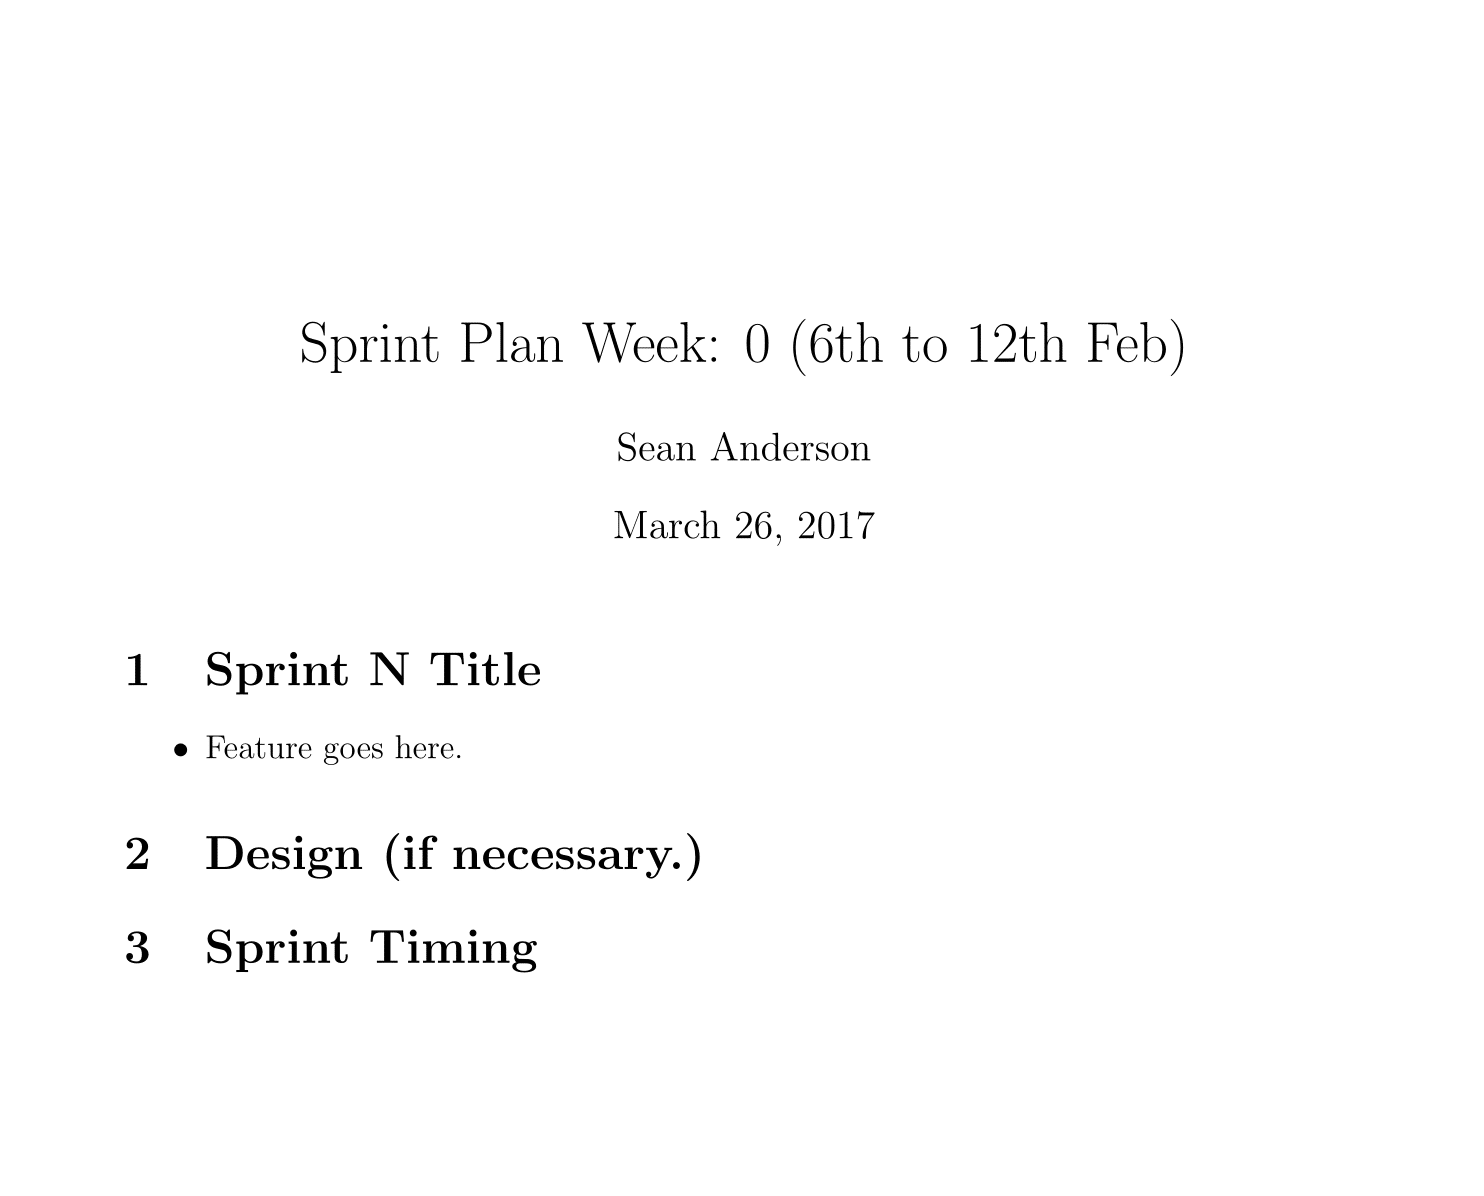
\includegraphics[width=\textwidth,height=\textheight,keepaspectratio]{images/sp}
\caption{The Sprint planning template}
\end{figure}
\begin{figure}[H]
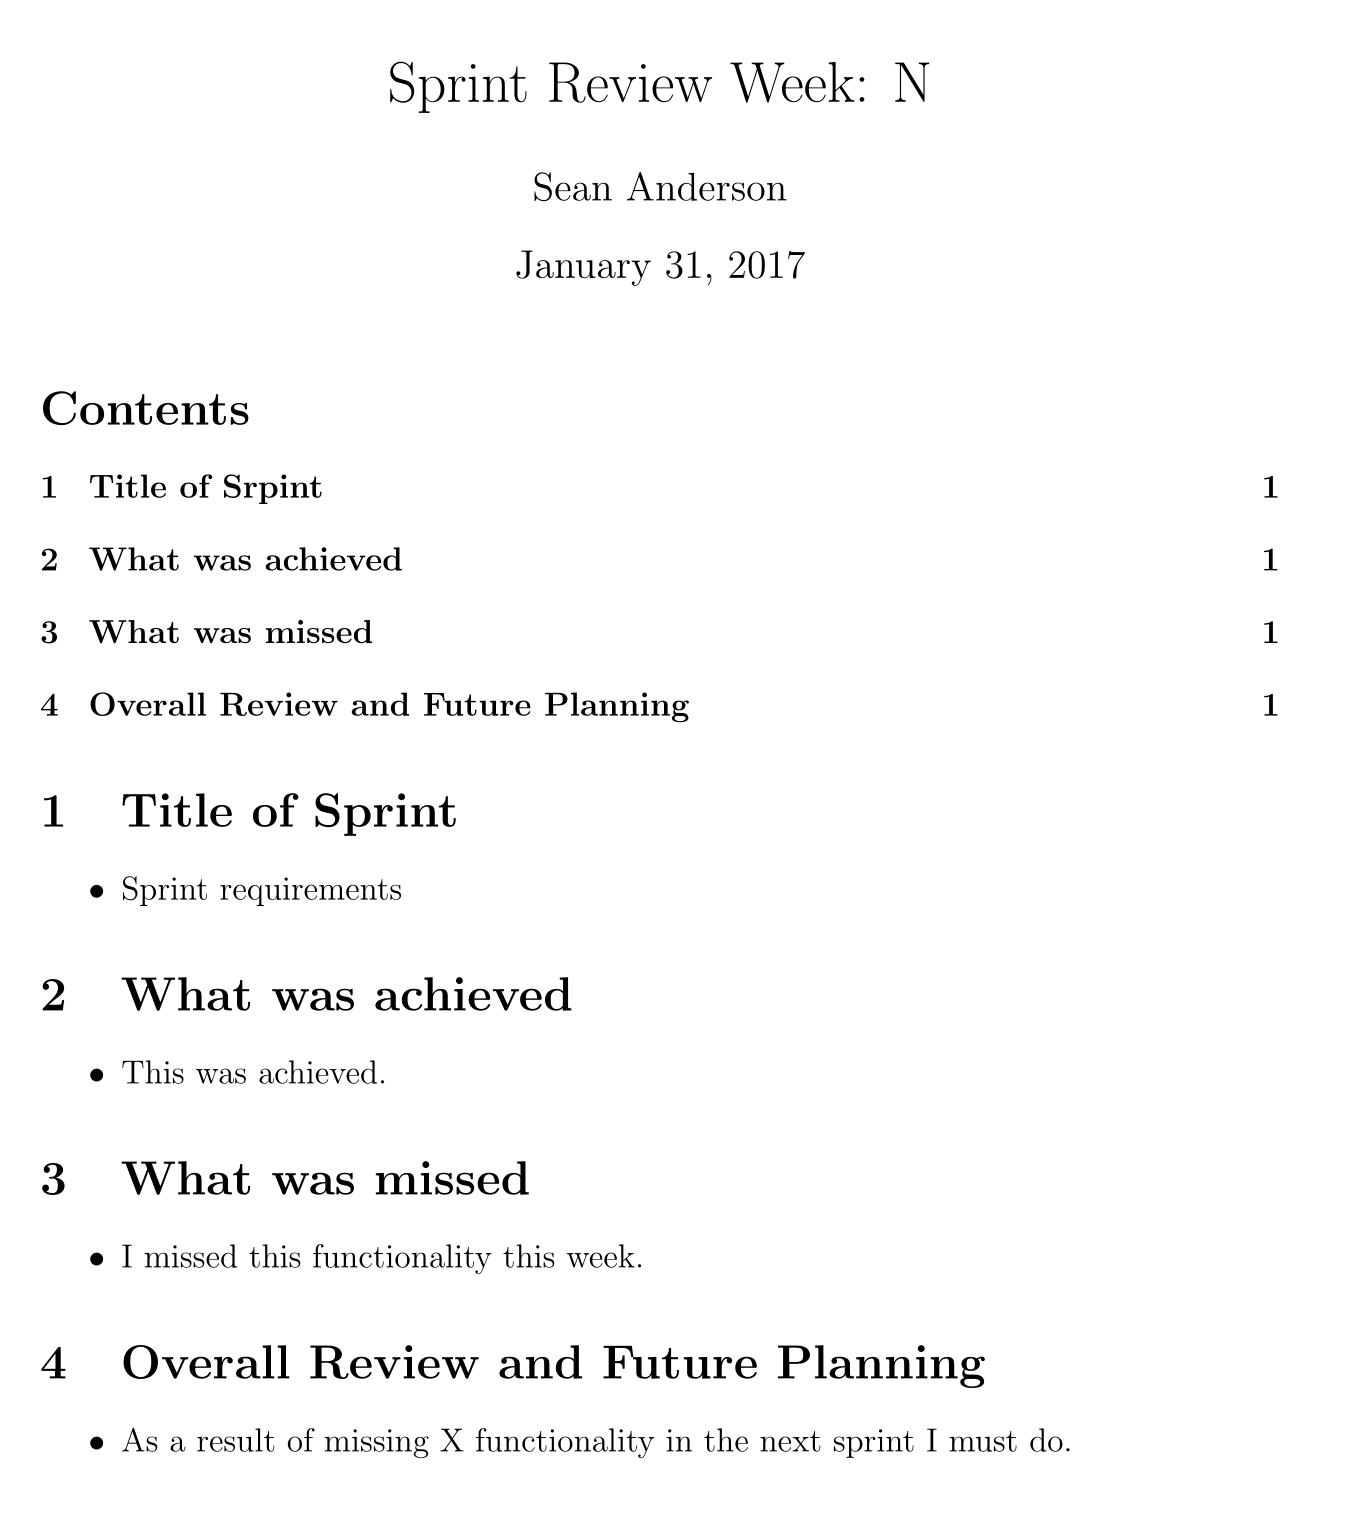
\includegraphics[width=\textwidth,height=\textheight,keepaspectratio]{images/sr}
\caption{The Sprint review template}
\end{figure}
\end{center}

\subsection{Initial Requirements}
Before splitting the different tasks into stories, it is important to consider the overall requirements of the system. Anyone must be able to register for an account; there will be three different types of account (a general music lover, an artist and a venue owner.) The general music lover should be able to follow artists and view events which are relevant to them. An artist should have the same functionality of a music lover however they will appear in a different section of the app. This is so it makes it easier for people to know who they are following. Both artists and music lovers should be able to post and people who follow them will see this post.

Venue owners need to be able to create events and add artists to these events. Music lovers should then be able to see all the appropriate information about these events. In terms of suggesting to the user who they should follow and what events they should attend, there will be some machine learning code placed on the back end of the system. As well as this the app, will need to be styled.

\subsection{Stories}
As Scrum is an agile methodology the project was split into multiple different stories. These include:
\begin{itemize}
	\item A register system so that all user types can create an account.
	\item A profile system which will allow for music lovers and artists to write a bio and upload a picture.
	\item A follow system so that users can follow other users.
	\item A post system so that when a user posts, all people who follow them can see that post.
	\item A create events system which can only be used by venue owners.
	\item Styling of the app.
	\item Recommendation system (which would be machine learning code) on the back end of the system which will mean users will get appropriate suggestions.
\end{itemize}

\subsection{Framework}
There are multiple different frameworks for developing apps using hybrid technologies. These frameworks all use web technologies however it differs from framework to framework as to what specific web technology is used. For example, apps made using the JQuery Mobile Framework are written in JQuery and apps made using the ionic Framework are written in AngularJS.

As well as considering the language of the framework it was also important to consider other factors before deciding which framework would be most appropriate. These factors include things such as page change speed, access to native APIs, external documentation and availability of community support.

Table 1.1 summarises information which was gathered from multiple resources and summarises  different hybrid app frameworks \cite{cordova} \cite{jquerymob} \cite{hab} \cite{cord} \cite{f7} \cite{ionic}.

 \begin{center} 
 \begin{tabular}{||c c c c||}
 \hline
 Framework Name & Summary & Advantages & Disadvantages \\ \hline\hline
 JQueryMobile & \begin{tabular}{@{}c@{}}Framework uses HTML, \\ CSS and JavaScript \\ \end{tabular}  & Simple to learn & \begin{tabular}{@{}c@{}} Limited plugins \\Page transitions \\ are slow \\Awkward to style \\ No longer a \\ large community \\ so lack of \\ support \end{tabular} \\
 \hline
 Phone Gap & \begin{tabular}{@{}c@{}}Framework uses HTML, \\ CSS and JavaScript \\ Built on top \\ of JQuery Mobile \end{tabular} & \begin{tabular}{@{}c@{}} Easy to learn -  \\ most developers  have \\ experience with \\ necessary languages \\ Many Plugins available for \\ access to platform's \\  native  APIs \end{tabular} & \begin{tabular}{@{}c@{}}Can be awkward to style \\ Page transitions can be \\ slow\end{tabular} \\ 
 \hline
 Ionic & \begin{tabular}{@{}c@{}}Framework uses HTML, \\ CSS (Sass if developer \\ prefers) and AngularJS \end{tabular} & \begin{tabular}{@{}c@{}} Simple to style \\  Large community support\\ Lots of plugins \\ Considered fast \end{tabular} & \begin{tabular}{@{}c@{}} Steep learning curve \\ requires developer to \\ understand AngularJS \end{tabular} \\ 
 \hline
Framework 7 & \begin{tabular}{@{}c@{}}Framework uses HTML, \\ CSS  and JavaScript \end{tabular} & \begin{tabular}{@{}c@{}} Easy to learn \\  Nice styling which\\ looks native \\ Can use in combination \\ with other frameworks \end{tabular} & \begin{tabular}{@{}c@{}} Not a very large \\ community so a \\ lack of support \\ Not many plugins \\ easily accessible by default \end{tabular} \\ 
\hline
\end{tabular}
\end{center}
 \captionof{table}{Table Comparison of Hybrid Frameworks}
\vspace{5mm}
Despite ionic having a steep learning curve due to it using AngularJS as opposed to JQuery it seemed like the most appropriate framework to use. This is because, not only does ionic have a fairly substantial amount of middleware plugins which allow for platform specific APIs to be accessed but it is also considered one of the fastest frameworks. This will aid the project aim of discovering whether hybrid apps are feasible alternatives to native apps. 


%\addcontentsline{toc}{chapter}{Development Process}
\chapter{Design and Experimental Methods}
\section{Design}
The ionic framework for developing mobile hybrid applications encourages the use of the Model View Controller (MVC) compound design pattern. MVC is something which is generally considered good practice within the software engineering industry and therefore the app was designed keeping that in mind.

The model of the app would be the database which is stored on the backend of the system. The view is the html files and the controllers are both the Angular JS controllers and the RESTful PHP API which I created.

\subsection{Overall Architecture}
The overall architecture of the system is complex and involves a lot of different files, this is due to the API which was created having over 35 PHP files which each perform specific tasks. Figure X shows the overall architecture of the system it doesn't go into each of the specific files however it does provide a good visual representation of the system.

\begin{figure}
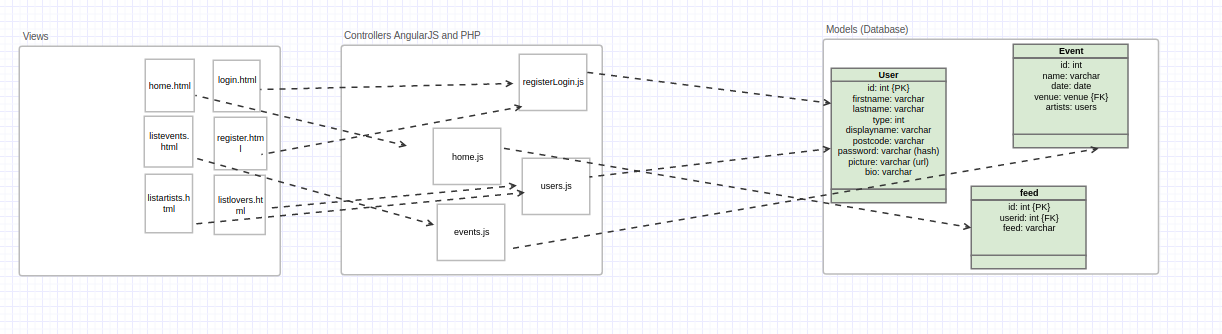
\includegraphics[width=\textwidth,height=\textheight,keepaspectratio]{images/overall}
\caption{Overall architecture of the system.}
\end{figure}



Figure 2.1 shows the system split into the front end view, controllers (which includes both the front end controllers (AngularJS controllers) and the API, PHP file controllers) and the model which is the database. This figure does not show every little detail of the system.


\subsection{Navigation System}
The navigation system is done mainly through view files, a controller is called by the menu. This controller then calls an API file to establish whether the user is a venue owner, if they are then it adds more links to the menu. Figure 2.2 (created using \url{https://www.lucidchart.com/}) shows this.

\begin{figure}[H]
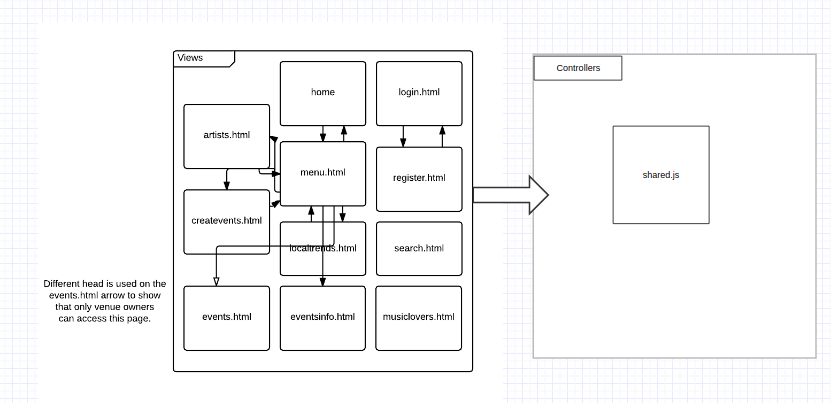
\includegraphics[width=\textwidth,height=\textheight,keepaspectratio]{images/systemdesign}
\caption{UML Diagram which illustrates the view}
\end{figure}

\begin{figure}[H]
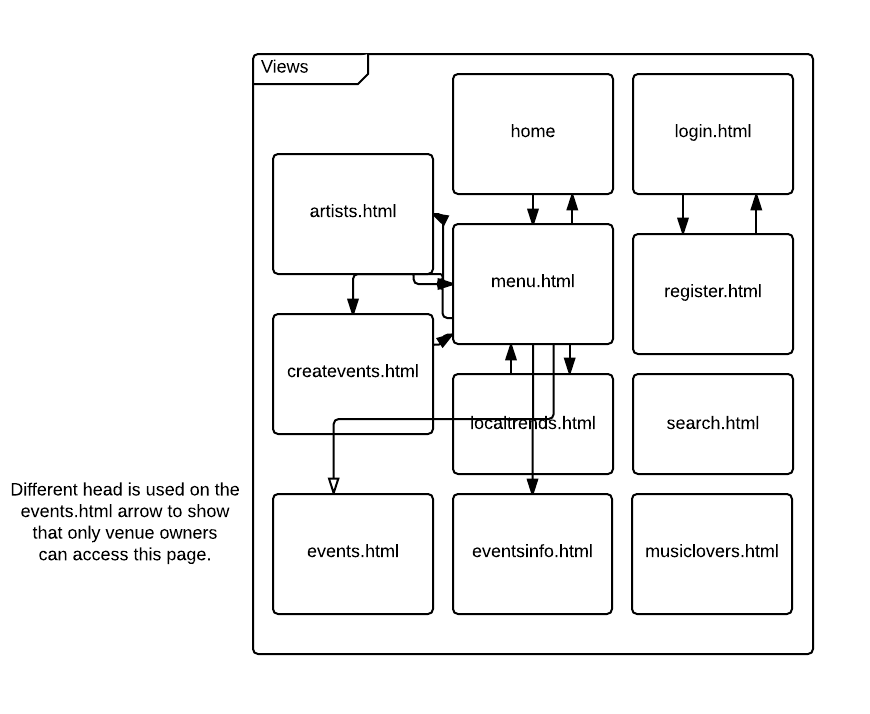
\includegraphics[width=\textwidth,height=\textheight,keepaspectratio]{images/va}
\caption{UML Diagram which illustrates the view interacting with controller.}
\end{figure}
Figure 2.3 shows just the view (created using \url{https://www.lucidchart.com/}) illustrates that once a user has logged in they can access multiple different pages through the menu bar (menu.html). The only page which is restricted is the events.html page as only venue owners can access this page to create events. The register.html page can only be accessed through the login page as it is accessed when a user needs to create a new account to login.

\subsection{Design of registration system}
The design of the registration system considered that there are three different types of user types. The music lovers and artists have the same details where as venue owners can also create events and venues. Figure 2.5 shows both the UML model for the registration system and the interaction between the model view and controllers.

\begin{figure}[H]
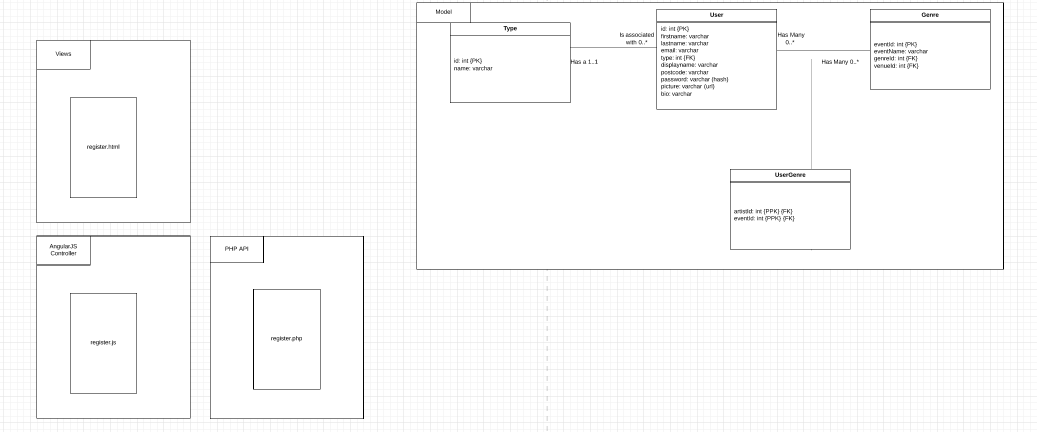
\includegraphics[width=\textwidth,height=\textheight,keepaspectratio]{images/register}
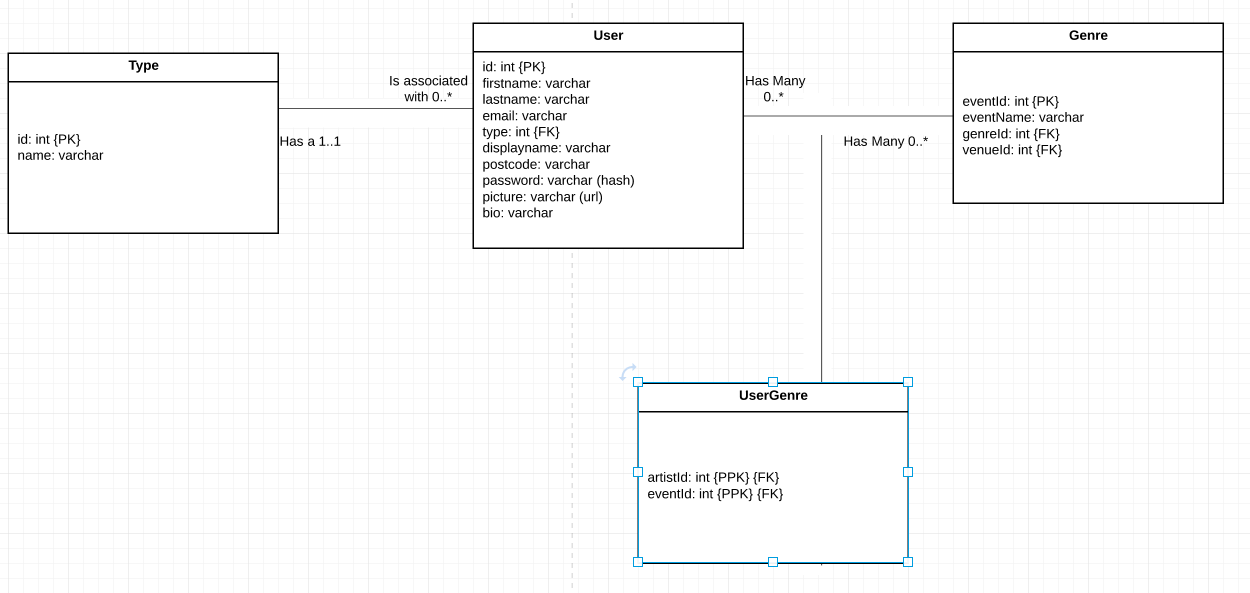
\includegraphics[width=\textwidth,height=\textheight,keepaspectratio]{images/users}
\caption{UML Diagram for the model in relation to a user registering.}
\end{figure}



\subsection{Design of events}

Figure 2.5 is a UML diagram (created using \url{Created using https://www.lucidchart.com/}) which shows the appropriate relationships between the different tables in the database in relation to an event. For the interaction with controllers etc. it works in the same way that the registration system does.
\begin{figure}[H]
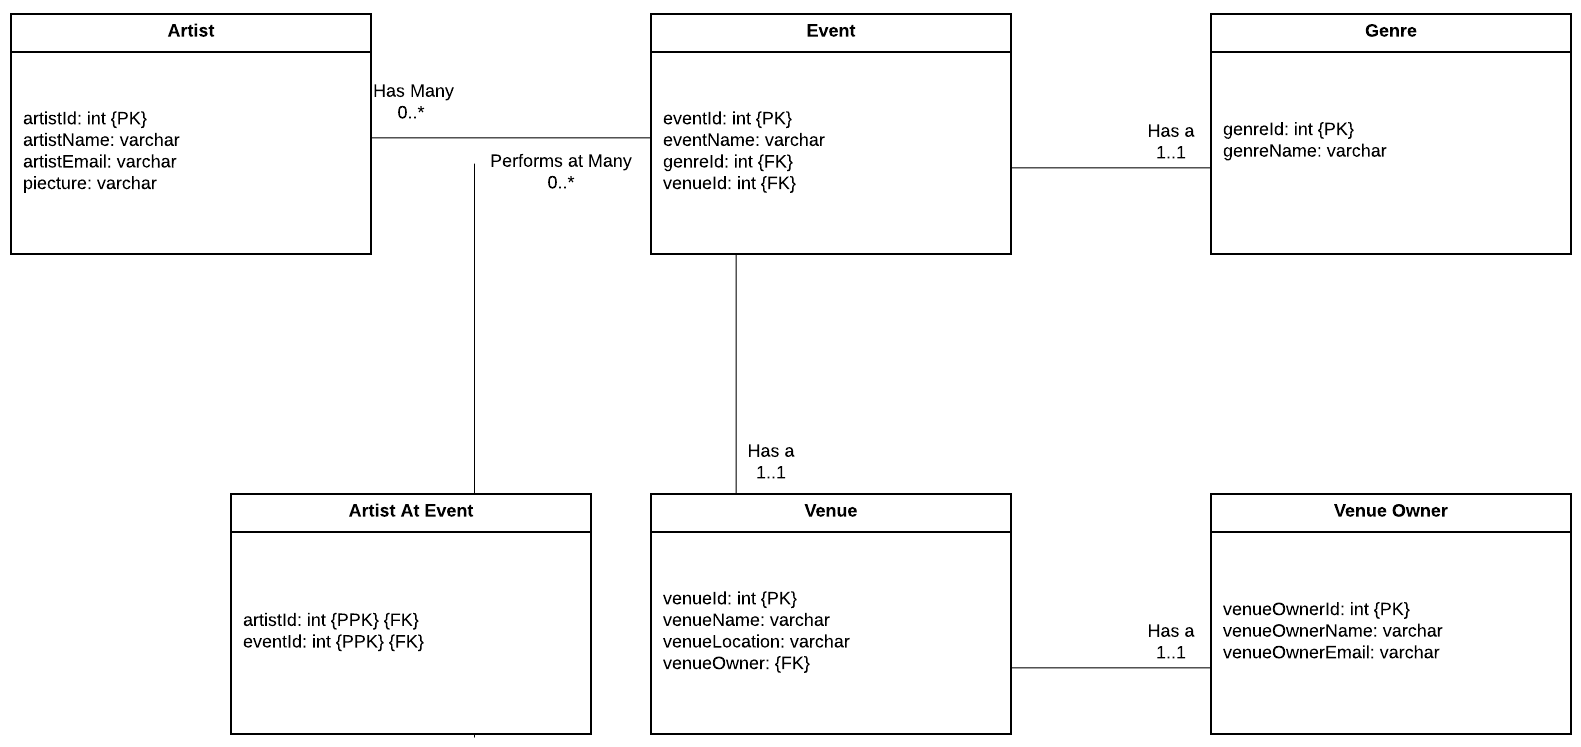
\includegraphics[width=\textwidth,height=\textheight,keepaspectratio]{images/events}
\caption{UML Diagram for the model in relation to events.}
\end{figure}


\subsection{User Interface}
In considering the music social network app it was decided that the name of the app would be Dynamic. Research into different social media sites was carried out and it was decided that blue would be the main colour used for the app, this is because blue is considered a relaxing colour and in terms of accessibility it is one of the most important colours.
\subsubsection{Shneiderman Principles} \cite{col}
Schniderman came up with eight golden rules for interface design, below the rules are listed followed by how they will be applied to the UI of the app. \cite{sch}
\begin{enumerate}
	\item 'Strive for consistency' - There will be a consistent colour scheme throguhout the user interface of the app, along with this navigation (where appropriate) will be the same throughout the app.
	\item 'Enable frequent users to use shortcuts' - There are multiple ways in which this can be applied to a mobile phone app. One way which it will be applied to the app will be allowing the menu (for navigation) to be opened simply by the user swiping the screen to the left. It will also be possible for the user to close the menu by them swiping to the right.
	\item 'Offer informative feedback' - Every time the user clicks a button on the app, the app provides them with feedback in a variety of ways such as by navigating to a different page or by a popup telling them the action they performed was successful.
	\item 'Design dialog to yield closure' - Popups were designed in such a way that the user can is notified of exactly what has happened and thus this will give them closure.
	\item 'Offer simple error handling.' - When things can go wrong for example if the user doesn't have GPS enabled they are informed of what the problem is and what a potential fix for the problem may be.
	\item 'Permit easy reversal of actions.' - The interface was designed so that the user can easily go back and change the options they selected.
	\item 'Support internal locus of control' - The interface has been designed so that the user is fully in control in terms of the data they are submitting and the way they are navigating between different pages.
	\item 'Reduce short-term memory load.' - The only thing which the user has to remember is there username and password to access the app.
\end{enumerate}
Figure X (created using \url {https://www.fluidui.com}) shows some UI mockups which were created.
\begin{figure}[H]
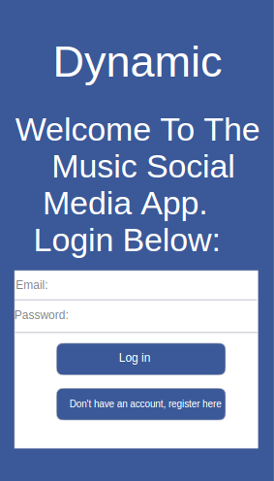
\includegraphics[scale=0.5]{images/ui1}
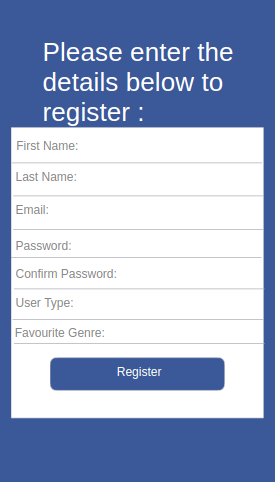
\includegraphics[scale=0.5]{images/ui2}
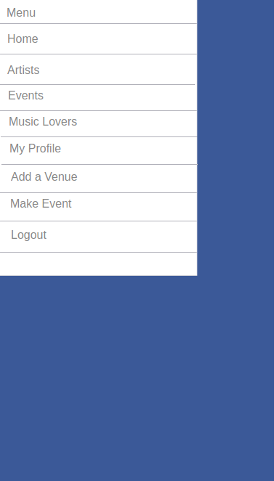
\includegraphics[scale=0.5]{images/ui3}
\caption{User interface mock up}
\end{figure}

\section{Experimental Methods}
As the purpose of the project was to determine whether hybrid apps are feasible alternatives to native apps tests had to be derived. User testing is key to this as it allows for general users (people who use apps on a regular basis) to give feedback about whether they think the hybrid app is as good as a native app, if not why not etc. Another key aspect to answering the question is comparing the resource usage on the device of the hybrid app to a standard app, this will include comparing things such as amount of RAM being used.

Finally ,during each story in the development process, it was considered whether using hybrid app technology was as challenging, more challenging or less challenging than developing using native app technologies.

\subsection{User Testing}
In establishing whether hybrid apps are feasible alternatives to native apps it was important to get general users thoughts about the app which had been produced. Within the development community there is a bit of a stigma associated towards hybrid mobile applications therefore in an attempt to remove bias the majority of people who fill in the questionnaires associated with the app will be lay people.

Whilst clearly it would be great to get a large amount of people to participate by filling in a questionnaire realistically only around 10 people were chosen. Before asking each individual questions, the project was explained to them.

The following questions were asked to each individual (a blank copy of the questions is in the apendix.)

\begin{enumerate}
\item On a scale of 1 to 10, with 1 being slowest and 10 being very fast in your opinion how quick is the app at processing the registration form?
\item On a scale of 1 to 10 with 1 being significantly slower than a native appm 5 being about the same time as a native app and 10 being significantly faster than a native app. In your opinion how quick is the app at processing the registration form?
\item On a scale of 1 to 10 with 1 being slowest and 10 being fast in your opinion how long does the process of uploading a profile picture take?
\item On a scale of 1 to 10 with 1 being significantly slower than a native app, 5 being about the same and 10 being very fast, faster than a native app. In your opinion how long does the process of uploading a new profile picture take?
\item On a scale of 1 to 10 with 1 being slowest and 10 being fast in your opinion how long does the process of viewing events and sorting them by using nearest events (GPS) take?
\item On a scale of 1 to 10 with 1 being significantly slower than a native app, 5 being about the same as a native app and 10 being very fast, faster than a native app in your opinion how long does the viewing events and sorting them by using nearest events (GPS) take?
\end{enumerate}
These questions were decided upon as they ensured that all of the stories which were relevant in terms of testing different elements of hybrid technologies can be tested.

\chapter{Implementation}
\section{Overall approach to implementation}
This chapter discusses the implementation of the music social network app 'Dynamic'. It is split into  multiple stories which have previously been listed in Chapter 1. Not all of the stories are discussed here as some stories were very similar to others.

\section{Toolset}
It was very important to use an appropriate toolset for this project. Using an appropriate toolset would not only save time but would also aid in the creation of code.

Git is one tool which was used throughout the creation of the project. Git is a very useful tool as it not only allows for just backups but also for version control \cite{git}. The main difference being version control means that all different revisions of the project could be viewed; this is extremely useful as it means that if the app code was to break, then the code could be restored to a working version. There are many different applications of git, consequently there are multiple providers of git services including Gitlab and Github \cite{github} \cite{gitlab}. For this project Github was used. As shown in Figure 3.1 a private git repository was set up which is what what used for version control and back ups.
\begin{center} 
\begin{figure}[H]
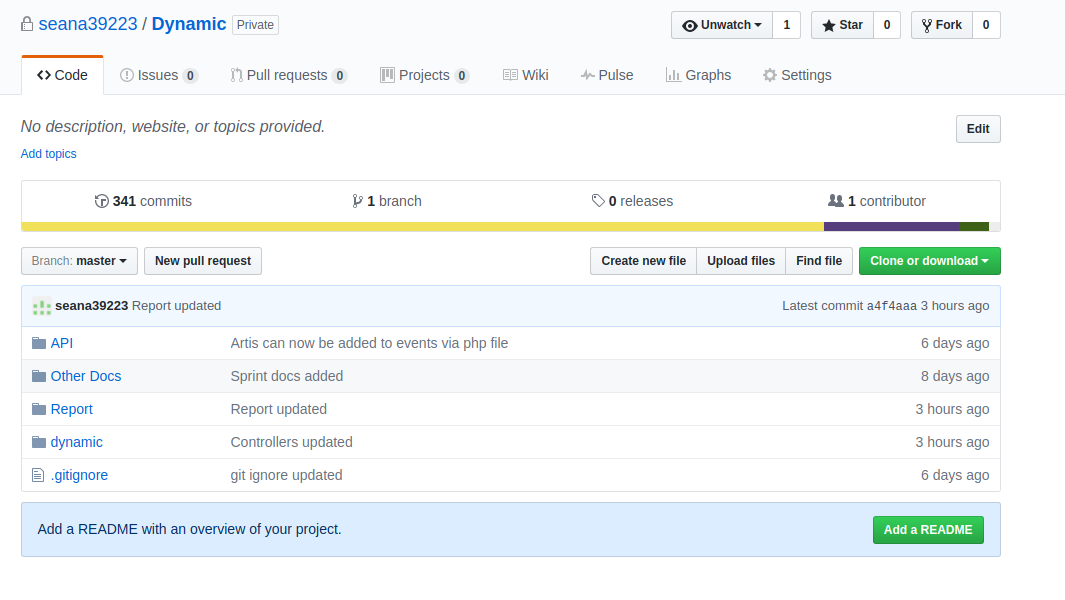
\includegraphics[scale=0.3]{images/git}
\caption{Git repository}
\end{figure}
\end{center}

Sublime is the text editor which was chosen for the project. Sublime was chosen as it has a large range of plugins, which are able to check the syntax of code along with tabulation etc. This is better than using a basic text editor such as vim as it makes producing the code easier.

\section{The Registration system}
\subsection{Back End}
Work began on the registration system by creating the appropriate tables in the back end database. These tables were user\_types, users, genres and user\_genres. The user\_types table contained the three different types of account which a user could have: Music Lover, Artist and Venue Owner and an id associated with each of these. The user type was implemented as a separate table to the users table itself for extensibility purposes as if additional user types needed to be added then they could simply be added to this table. The users table just contained all of the users' details including name, display name, email, password (discussed in more depth during the security section) and a url link to their profile picture. The genres table was simply a table which contained different genres of music and an appropriate id for each genre. As genres to users is a many to many relationship a users\_genres table was created which stores a user\_id and a genre\_id.

After the tables had been created, the php files (hosted at \url{seananderson.co.uk/api}) were created. These php files essentially formed the RESTful API which would allow for the front end to connect to the database for this system. The first file which was created was register.php. This file takes variables which the user passes in (through POST data) and adds them to the database via my sqli commands which are run from within the php. This file automatically gives the user a generic picture url of a gingerbread man \cite{ginger}. Some validation was done in the php file to check that things such as emails given are valid email addresses, however most of the validation was done on the front end as this would allow for error messages to reach the user in a quick manner. 

As at this stage in time there was no front end, consequently it was not possible to test that sending POST data from the app would work. So, a piece of software called postman (which is a Google Chrome extension) was used. This software allows for POST data to be pushed to a website or API as illustrated in Figure 3.2. As well as relying on the PHP file telling me 'A new user was added successfully' which is the message what is printed when the sql commands all run correctly, the database was also checked to ensure that the new user had been added correctly as shown in Figure 3.3.

\begin{center} 
\begin{figure}[H]
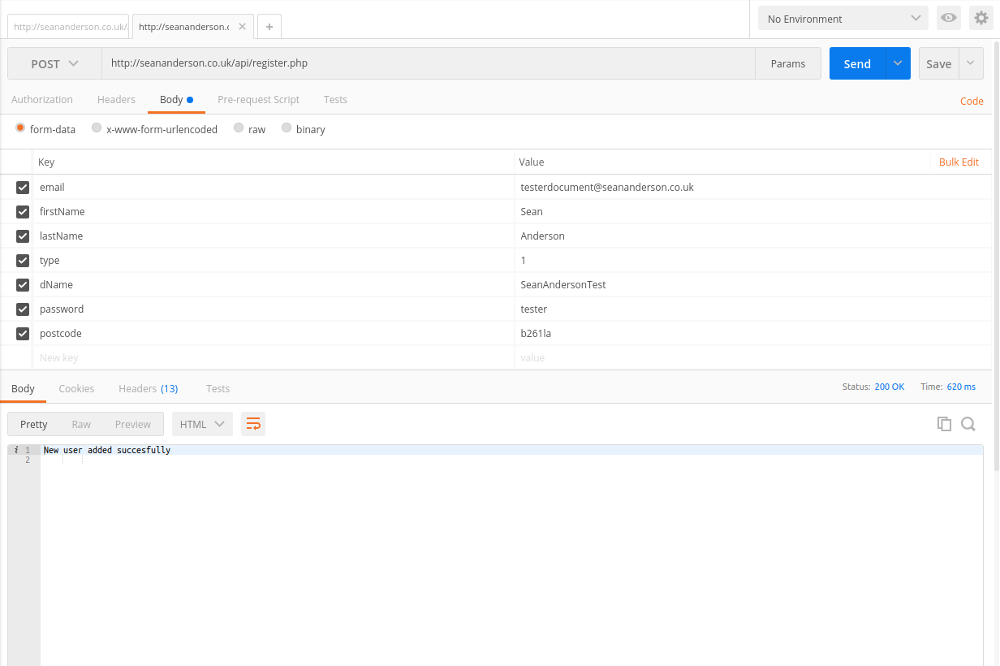
\includegraphics[scale=0.45]{images/postman}
\caption{Postman testing register.php}
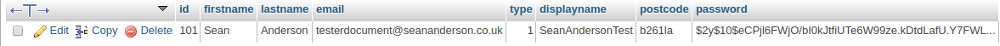
\includegraphics[scale=0.45]{images/db1}
\caption{User added to the database}
\end{figure}
\end{center}

\subsubsection{Security within the registration system}
It is important that users are not allowed to enter dangerous characters into the database, as a result of this all strings which are inputted by the user are escaped using the mysqli\_escape function which is a default php function which ensures that any characters which could potentially do damage to the database are escaped and therefore not ran in the mysqli statements.

As the registration and login system used a password it was important to ensure that if somebody was to get access to the database that they wouldn't get access to the password. There are multiple different methods of encryption which could have been used for this. PHP has its own built in function called password\_hash which takes in two parameters the password itself as a string and the encryption type. For this project password\_default which is a predefined php hashing method was used. Password default was used as it was a simplistic and relatively secure way of turning a password into a hash. The password\_verify function in PHP is used to check that a plain text password matches the hashed password.
 
\subsection{Front end}
After the back end for the registration of the app was created, development then started on the front end. The default ionic menu bar template was used as this would allow for a menu bar to appear on multiple pages (like in the design) easily.

The views for both the login and registration system were created using html (as are all views in ionic) and the controllers for these views were created in AngularJS and were simply js files. Both the register and login view files contained a form which gathered appropriate information from the user and then passed that information onto the controllers when submitted. The controllers then passed that information onto the API's by using \$http.post which is an AngularJS method used for calling post API's. Figure 3.4 shows how the AngularJS controller passes the appropriate data to the API. The full code for the registration system is shown in Appendix 3.
\begin{center}
\begin{figure}[H]
\begin{verbatim}
$http.post(api, data).then(function(res){
  apiReturns = JSON.stringify(res);
  if (apiReturns.includes('New user added succesfully')>=0) {
    localStorage.setItem('email', $scope.register.email);
    localStorage.setItem('dName', $scope.register.dName);
    if ($scope.registerGenre!=undefined) {
      $scope.registerGenre();
    }
    $state.go('app.profile');
    popUp('Welcome', 'Welcome to Dynamic please fill in 
    your profile page and then follow some users');
  }
})
\end{verbatim}
\caption{AngularJS code for posting to register account}
\end{figure}
\end{center}

In passing the information from the controller to the API I encountered a problem. AngularJS sends post data in a different way to most other languages. As a result of this the following lines of code had to be added to the PHP files as shown in Figure 3.5. (This code was taken from \url{http://corpus.hubwiz.com/2/angularjs/15485354.html})
\begin{center} 
\begin{figure}[H]
\begin{verbatim}

if ($_SERVER['REQUEST_METHOD'] == 'POST' && empty($_POST)) {
    $_POST = json_decode(file_get_contents('php://input'), true);
}
\end{verbatim}
\caption{Code to make API work properly}
\end{figure}
\end{center}

Figure 3.6 shows what the front end for the login and registration screens look like on the front end on the system (from the perspective of a One Plus Two device.)
\begin{center}
\begin{figure}[H]
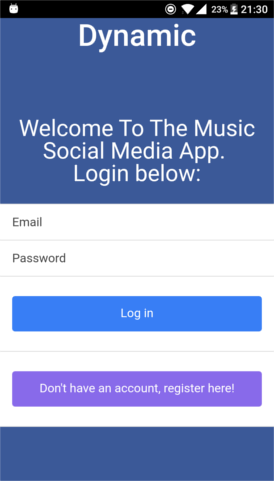
\includegraphics[scale=0.5]{images/sc1}
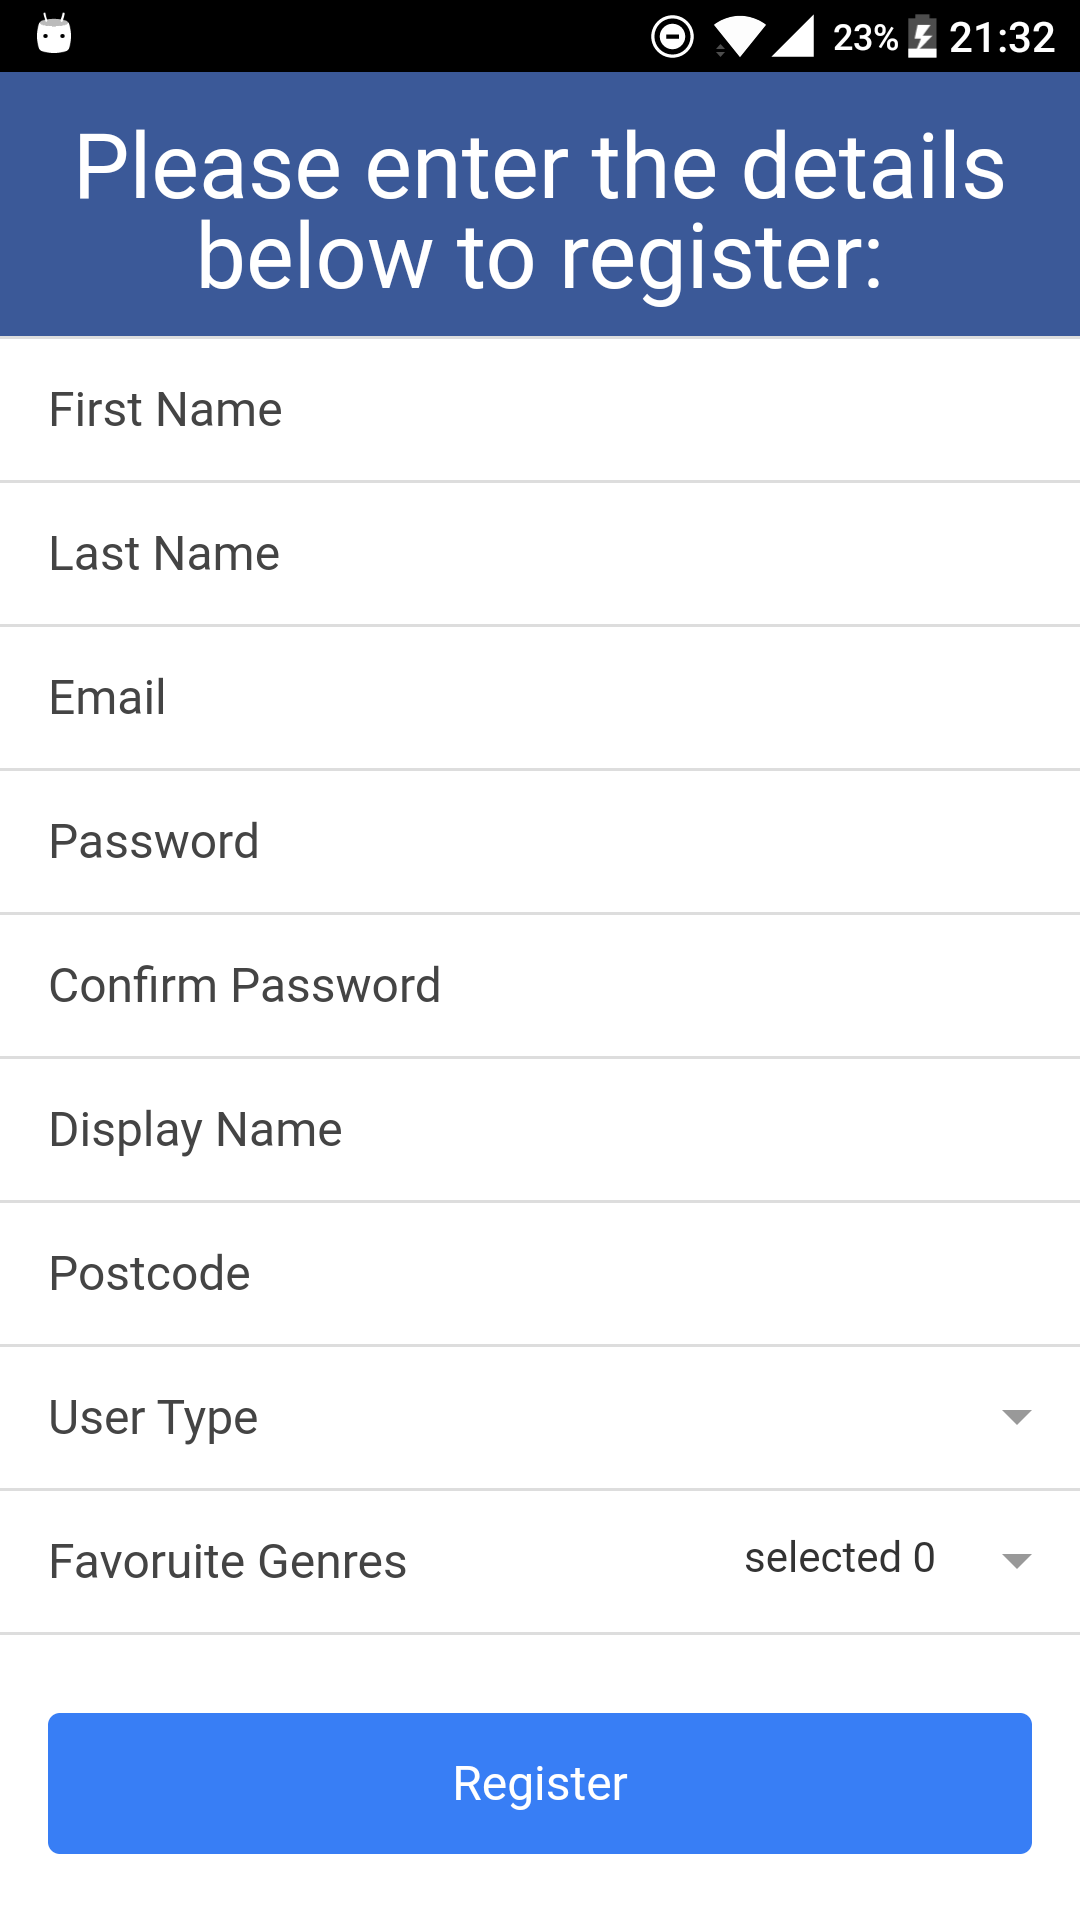
\includegraphics[scale=0.5]{images/sc2}
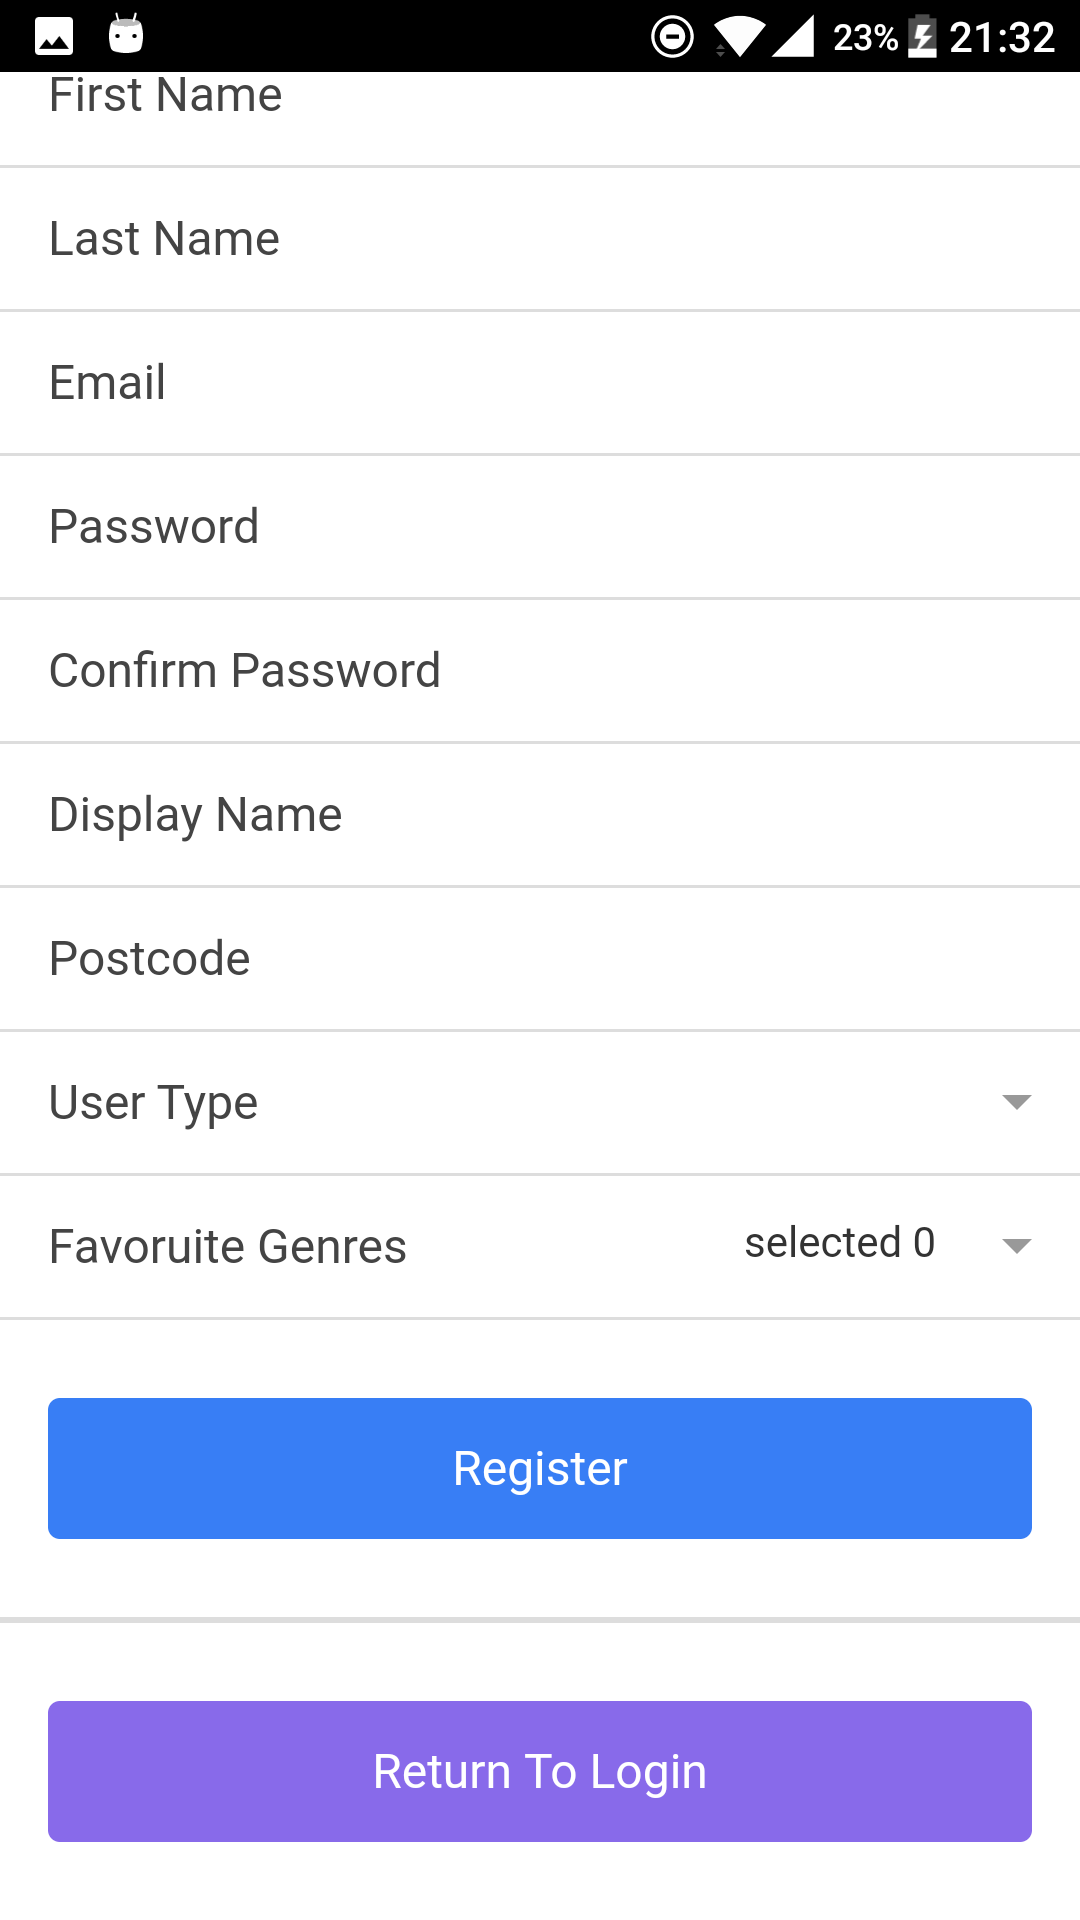
\includegraphics[scale=0.5]{images/sc3}
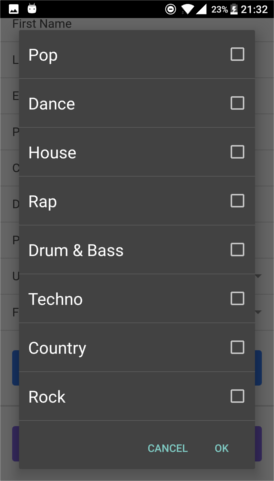
\includegraphics[scale=0.5]{images/sc4}
\caption{Screenshots of registration system.}
\end{figure}
\end{center}

\subsection{Validation}
Having successfully got the front end interacting with the back end it was important to ensure that all of the data being sent over was valid. I decided first of all to validate the data on the front end. This ensured that the user had filled in all of the appropriate boxes and a regular expression was used to ensure that the email address they entered was valid.

It was then necessary to create some more API files as each user had to have a unique email and display name, files called checkemail.php and displayname.php were created. These files run SQL queries to ensure that the email address and display name which the user entered are unique.

Figure 3.7 displays an example of what happens when a user tries to register an account with an email address which has already been used and when a password is not long enough.
\begin{center}
\begin{figure}[H]
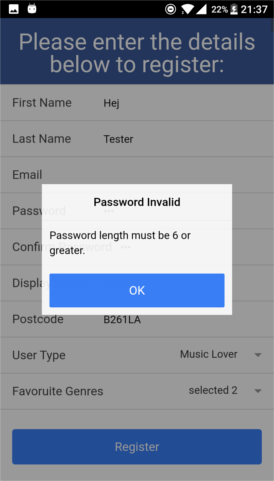
\includegraphics[scale=0.5]{images/sc5}
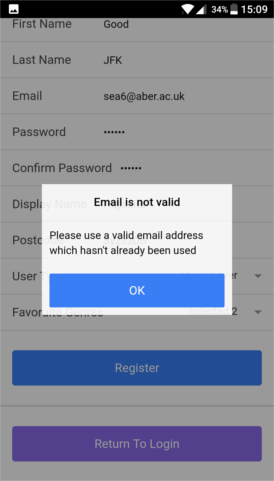
\includegraphics[scale=0.5]{images/sc6}
\caption{Validation Screenshots}
\end{figure}
\end{center}

\section{Posting to a feed}
There were multiple ways in which a user posting to a feed could be carried out. It was decided that a users posts would be stored in the database and would be retrieved from the database at appropriate times. As the relationship between a user and a post is a many to many relationship, a new table was created in the database called feed. 

An API file called feed.php was created, this file takes in two post variables a users email and a users post (the string the user would like to add to their feed.) This file then uses the users email and runs a sql command to get the users id. This id is then placed into the feed table along with the users post variable.

The front end of the system worked in a way which was very similar to the registration system. The view of the front end was simply a text input field and a button (as shown in Figure 3.8) which when clicked would call an action in the controller.

This controller would then pass the appropriate variables to the API, using \$http.post in the same way as the registration system. Finally a message would display to the user to let them know they had posted, this is shown in Figure 3.8.
\begin{center}
\begin{figure}[H]
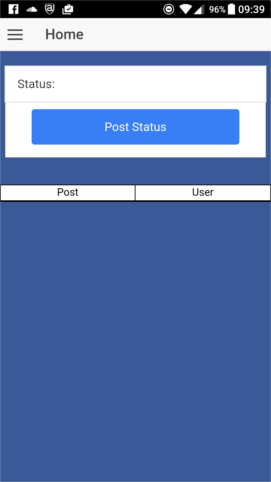
\includegraphics[scale=0.5]{images/sc10}
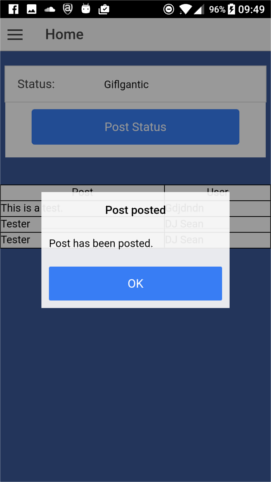
\includegraphics[scale=0.5]{images/sc11}
\caption{Validation Screenshots}
\end{figure}
\end{center}

\section{Creation of Events}
An important component of the mobile application was that users with the type venue owner could create events. Creating events is split into two different parts, actually adding the venue where events will take place to the app and then the actual creation of an event.

\subsection{Adding a Venue}
The purpose of adding a venue to the app is so that a venue owner can quickly create multiple events at the same venue and they don't have to enter the venue's details every time. The system for adding a venue was designed in a way that should be simple for the venue owner to add a new venue. They simply had to navigate to the 'Add a Venue' page and enter the appropriate details as shown in Figure 3.9. 

The system worked in the same way as the registration system in how it passes the data to the back end.
\begin{center}
\begin{figure}[H]
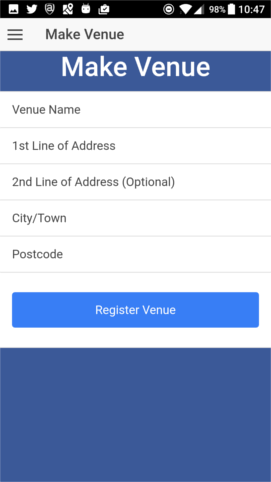
\includegraphics[scale=0.5]{images/sc12}
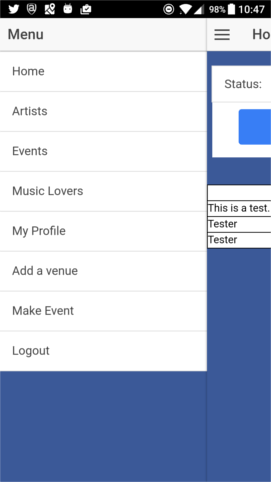
\includegraphics[scale=0.5]{images/sc13}
\caption{Front End for adding a venue}
\end{figure}
\end{center}

\subsection{Adding an Event}
Adding an event requires the user to already have a venue associated with them, consequently a message is displayed telling the user to add a venue if they don't already have one as shown in Figure 3.10.
\begin{center}
\begin{figure}[H]
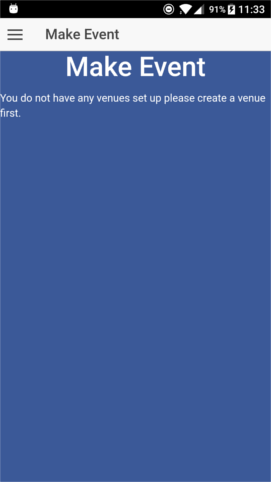
\includegraphics[scale=0.5]{images/sc14}
\caption{Message which displays if the user has no venue.}
\end{figure}
\end{center}

Then once the user has created a venue they can create an event. The user simply fills in the appropriate details to create an event. The three drop down options on the page event venue, closest genre of event and artists performing are populated through API's. In terms of the event venue an API is called which gives all of the venues associated with the user logged in. The closest genre of the event is simply all of the genres which are in the database and the artists performing at event is made up of all artists who have an account on the app as shown in Figure 3.11. Once the details the user has entered are validated, in that all of the information they have provided is valid (correct) the event is then added to the app and both music lovers and venue owners can add events to their favourites. 
\begin{center}
\begin{figure}[H]
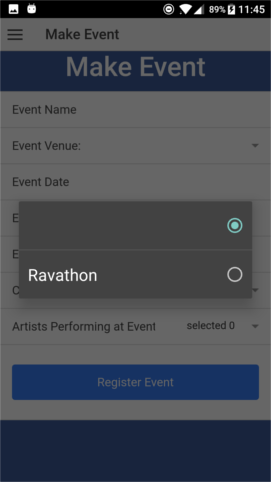
\includegraphics[scale=0.5]{images/sc16}
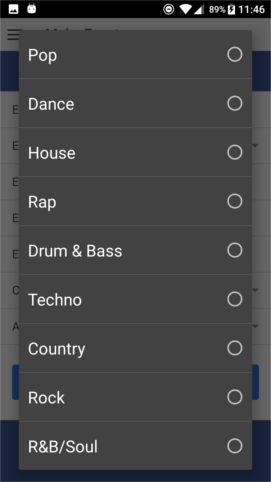
\includegraphics[scale=0.5]{images/sc17}
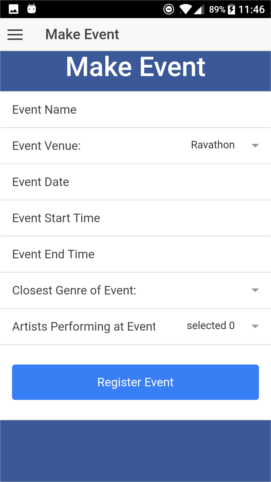
\includegraphics[scale=0.5]{images/sc18}
\caption{Creating an event}
\end{figure}
\end{center}

\section{Users profile}
Having created the registration and login system the next story which was tackled was allowing the user to add a bio and to upload a picture. This picture would act as the users profile picture. Having previously completed the registration system allowing the user to add a bio was rather straightforward. It was just simply a matter of creating a front end which passes a variable to a php file (called update bio.php), the php files then takes the post variable and turns it into a php variable. Finally as shown in figure X the php file runs a sql command which updates the users table to have the correct information for the bio.

\begin{figure}[H]
\begin{verbatim}
$sql = "UPDATE users SET bio = '$bio' WHERE displayname = '$dName' ";
\end{verbatim}
\caption{Snippet of updatebio.php code which shows SQL command.}
\end{figure}

\subsection{Camera and FileTransfer plugins}
The task of allowing a user to upload a profile picture can be broken down into two seperate tasks. The task of actually allowing the user to take the photo or pick a photo from their devices library, and the task of transferring that photo to the back end. 

Installing the cordova camera plugin \cite{cc} was necessary to allow the user to take a photo or select a photo from their devices library. The actual installation of the plugin was simple, following the documentation for the plugin was straightforward and the app was programmed so that if the user clicked a button saying upload a picture or choose a picture from my gallery then the Cordova Camera plugin was called with the correct options configured.

Figure 3.12. highlights the two different buttons and what happens when they are clicked.
\begin{center}
\begin{figure}[H]
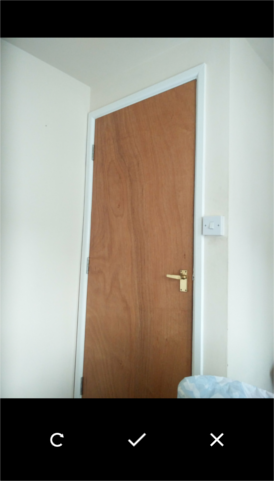
\includegraphics[scale=0.5]{images/cs}
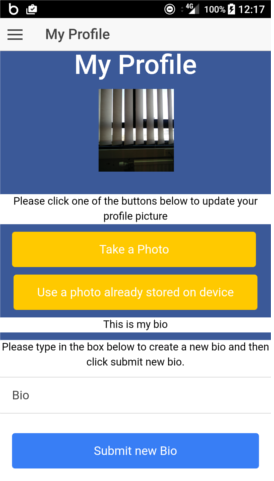
\includegraphics[scale=0.5]{images/sc7}
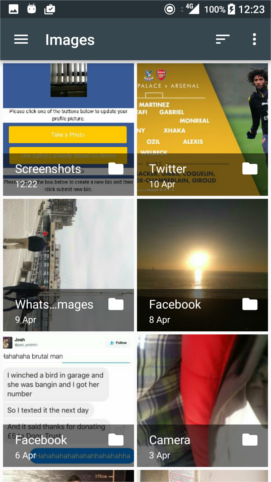
\includegraphics[scale=0.5]{images/sc9}
\caption{Screen shot of camera functionality.}
\end{figure}
\end{center}

After the user confirms (by pressing the tick) that they want to use the photo as their profile picture the photo is then uploaded to the server. The first step in getting the photo to upload was to create a API file, this file was entitled imageupload.php and is hosted at \url{seananderson.co.uk/api/imageupload.php}. This file contains some fairly trivial code which just gets the data of the image which has been uploaded and places it in an appropriate folder (\url{seananderson.co.uk/api/uploads}). After creating the php file the next step was to pass the photo from the device to the server. This was done by using the Cordova File Transfer plugin \cite{ft}. This plugin simply takes a file (which in this case was the image) and uploads the file to the specified URL.

After implementing the camera plugin one clear disadvantage of hybrid apps became apparent. The time taken for the device to take a picture and then process that picture was noticeably longer than it takes when using a native app such as Facebook. This is discussed in more depth during the testing section of this report. 

\subsection{Caching issue}
At this stage of the development of the app it became apparent that there was an issue with caching. The issue was when the picture was loaded onto the users profile page after the user uploaded a new picture, the picture would not be updated and would display the users old display picture even though the new image had successfully been uploaded. 

A variety of different ways were used to try and tackle this issue. Ionic allows for the apps cache to be cleared using \$ionicHistory.clearCache(); however this unfortunately didn't resolve this issue. As clearing the apps cache wasn't getting rid of the issue it was clear that the problem lay within the browser (which is how the app is ran.)

It turned out that the Chrome browser was caching the results of the API which displayed the picture, as the same API was being called on the page refresh, which was ran once the photo was uploaded. Despite not being the most elegant solution a random number was added to the end of the pictures url as shown in Figure 3.13.
\begin{center}
\begin{figure}[H]
\begin{verbatim}
$http.post(api, data, { cache: false }).then(function(res){
  //Below line is a hack, justified in report.
  var image = (res['data']['picture']) + '?random=' + Math.random();
  var photoDiv = angular.element(document.querySelector('#profile-photo'));
  photoDiv.html('<div id ="profile-photo"><img  height="60 px" 
  width="60 px" src="' + image + '"</img></div>');
})
\end{verbatim}
\caption{AngularJS Photo Code.}
\end{figure}
\end{center}

This meant that the browser would load the new image uploaded into the app as it would have a different url from the old image. The caching issue is clearly a negative to hybrid app development, if the app was developed in a native manner then it would allow for the developer to have full control over the cache and therefore this issue would not have arose had the app been developed in a native manner. 

\subsubsection{Problem with Different Devices}
The camera plugin worked fine on a One Plus Two mobile phone, however when the camera was tested using a Samsung Galaxy A there was a problem, the orientation of the image was wrong. The Samsung Tablet would take the photo fine but when it actually came to uploading it, it would rotate the image. 

One of the options when using the camera plugin is photo orientation as shown in Figure 3.14. 
\begin{center}
\begin{figure}[H]
\begin{verbatim}
var options = {
  quality:80,
  targetWidth:500,
  targetHeight:750,
  sourceType : Camera.PictureSourceType.CAMERA,
  encodingType: Camera.EncodingType.PNG,
  correctOrientation: true
};
\end{verbatim}
\caption{Camera Plugin Options.}
\end{figure}
\end{center}
Unfortunately enabling that to be true still didn't solve the problem. Despite there not being any official sources suggesting why the correct orientation doesn't always work the feeling within the Ionic Community is that Samsung devices actually ignore the correctOrientation option \cite{ioniccom1}. This is clearly another disadvantage to hybrid apps as native apps would give the developer more control \cite{androidcamera}.
\section{Styling and porting over to iOS}
As ionic uses HTML for its views, the styling is done in CSS, SASS can be used as an alternative to CSS if the developer wants. The majority of the app was styled whilst working on each story however it was important to spend some time to ensure that the styling of the app was consistent across multiple devices and platforms.

iOS mobile applications can only be released and launched through using xCode which is only available on Macs. Clearly this requires some effort however it requires significantly less effort than if the apps were developed in a native manner. If the apps were developed in a native manner then the code would have to be completely rewritten for launch on iOS devices where as when using a hybrid technology it is simply a matter of installing any plugins on the Mac which were installed when developing the Android version and potentially some slight tweaks to the styling as Android and iOS browsers interpret CSS slightly differently. 

This did actually bring up some issues with hybrid app development. Whilst a key feature of hybrid app development is the ability to deploy an app to multiple different code bases; iOS and Android interpret CSS differently. Therefore time had to be spent tweaking the CSS of the iOS version. (Add this if possible Figure X shows a particular part of the app running on iOS and Android however it is clearly inconsistent.)

\begin{figure} [H]
\caption{iOS not the same as Android image goes here}
\end{figure}


\section{Recommendation System}
When creating the recommendation system it was considered that information about the user to recommend events can be obtained explicitly and implicitly \cite{ML}. It was important to consider that if the app was released commercially then the ethics of obtaining data implicitly would need to be considered and the user would need to understand exactly how their data would be used.

The recommendation system was made for events and in terms of explicit data available, two pieces of information were relevant these were the users favourite genre's of music and the users postcode. This is because each event has a genre associated with it and a postcode so comparing this information allows for the establishment of how similar in terms of music the user likes is to the event and the distance between the user and the event. When using the explicit data to recommend events the system would be using content based filtering \cite{san}.

There was only one relevant type of implicit data available about users which would help in creating a recommendation system, this is the users current favourite events. If the user has already chosen to favourite a event then it is possible to compare the events they currently have favourite with other events and make recommendations based of how similar the events are. When using implicit data to recommend events the system would be using collaborative filtering algorithms \cite{collab}.

\subsection{Content Based Filtering}
The recommendation system runs when the user decided to sort events by recommended events. The first thing which happens when the user does this is that the app makes a call to the back end which checks if the user has any events in their favourites. If they do have events in their favourites then the system uses collaborative filtering algorithms to recommend events if not it uses the following method to recommend events using content based filtering.
\begin{enumerate}
  \item Looks up genres of music associated with the user.
  \item Looks to see if any of those genres of music are being played at events and adds appropriate events to an array.
  \item Sorts the array in terms of distance between the users home and event.
  \item Displays the recommended events on the app itself.
\end{enumerate}
Figure X shows how steps 1 and 2 work via php code (the full code can be seen in Appendix 4 under recommendedevents.php).
\begin{figure}
\begin{verbatim}
$sql = "SELECT genre_id from user_genres WHERE user_id = '$userId'";
$genres = $connection->query($sql) or trigger_error($mysqli->error."[$sql]");
    foreach ($genres as $genre) {
        $genreIdSql = $genre['genre_id'];
        $sql = "SELECT * from events WHERE genre_id = '$genreIdSql'";
        $events = $connection->query($sql) or trigger_error($mysqli->error."[$sql]");
        while($event = mysqli_fetch_assoc($events)) {
            $eventsArray[] = $event;
        }
    }
}
\end{verbatim}
\caption{Code which shows how steps 1 and 2 work for Content Based Filtering}
\end{figure}
Figure X shows how the events display on the front end of the app once they have been sorted.
\begin{figure}
\caption{Insert figure showing sorted events here.}
\end{figure}

\subsection{Collaborative filtering}
When the user does have some favourite events, collaborative filtering is performed to give the user recommended events. As with the content based filtering this process was split into multiple steps.
\begin{enumerate} 
  \item All of the users favourite events are added to an array.
  \item An empty array is created called recommended events.
  \item A calculation is then performed to calculate the similarity between the events which the user hasn't got as favourites and the events they have got as favourites.
  \item Events which the user doesn't have as favourites are added to the recommended events array in order of how similar they are to the events which the user has already placed as favourites.
\end{enumerate}
The calculation for similarity between events consists of two main things; the genre of the event and the location of the event. This calculation is essentially an implementation of the K Nearest Neighbour(k-NN) machine learning algorithm \cite{knn} \cite{knn2}. K-nn is a useful machine learning algorithm which can be used to classify data, it was implemented in such a way to this project so that an event which is near to an event which a user is attending would be a recommended event to a user.

\section{Debugging and other features of hybrid app development}
One massive advantage of the ionic framework is that the developer can actually launch the app in a Google Chrome browser by running the 'ionic serve' command from a terminal. This is a very useful feature as it also allows for code to be edited and the page will simply refresh as shown in Figure 3.15. This is a clear positive of hybrid app development as it means that the code can be 'live edited' so the developer can see the changes they are making and because the user doesn't necessarily have to use emulators which can be resource heavy.
\begin{center}
\begin{figure}[H]
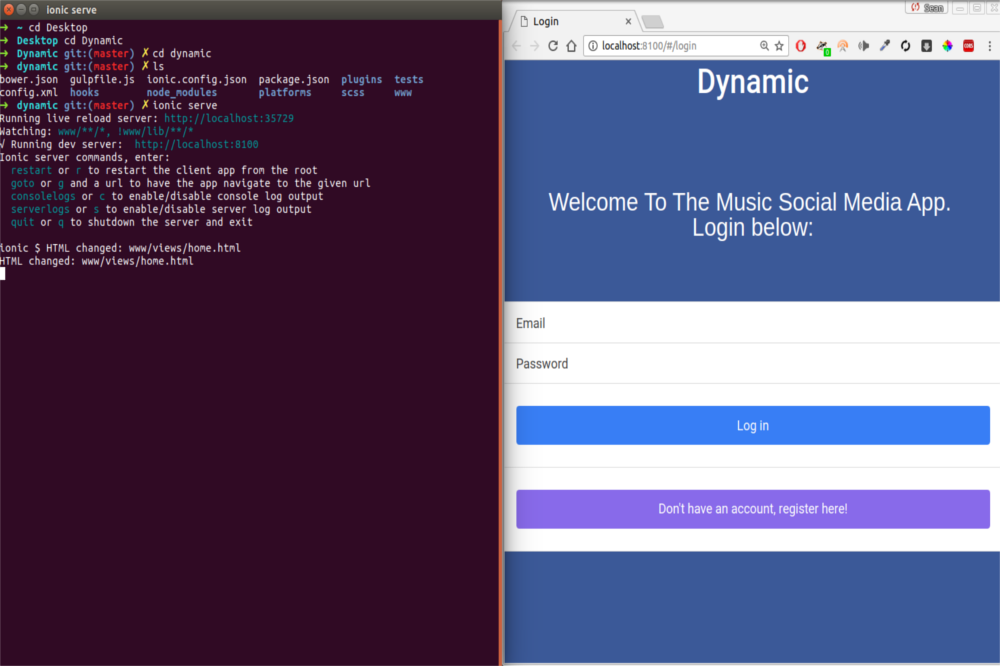
\includegraphics[scale=0.45]{images/chrome}
\caption{ionic serve command running}
\end{figure}
\end{center}

Debugging the app is also rather straightforward as Google Chrome's developer tools can be opened up whilst running ionic serve as shown in Figure 3.16 this allows for various commands to be typed to test a variety of things and also for console logs to be displayed which clearly aids the developer in checking variables.
\begin{center}
\begin{figure}[H]
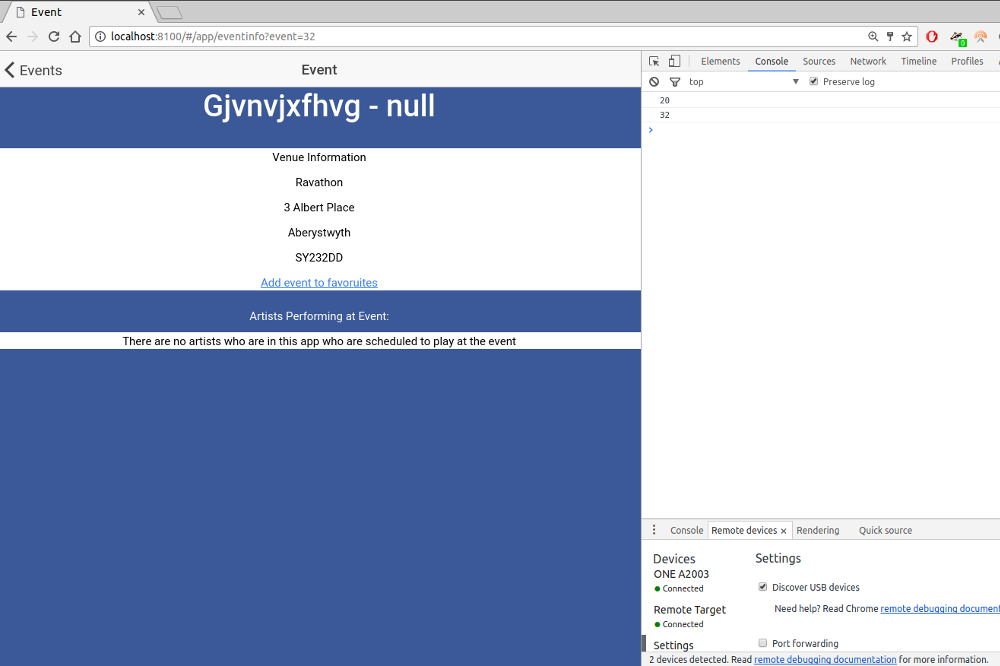
\includegraphics[scale=0.45]{images/chrome2}
\caption{Chrome developer tools}
\end{figure}
\end{center}

\section{PHP files}
The back end of the app had over 30 PHP files, this had clearly taken a lot of time to develop. There is a lot of overlap in the files and a lot of them are very similar they just perform slightly different functions. When the system was initially thought of it wasn't expected that there would be so many PHP files and that is why all of the files were wrote manually, rather than using a framework. 

This is where using an agile approach for the project had a negative impact, as if a plan driven approach had been used then it would have been realised much earlier on in the project the sheer amount of PHP files which would have to be created and so an appropriate framework would have been selected.

\section{Technical challenges}
There was multiple technical challenges which were faced when developing the app. The first of which was actually learning AngularJS, this was simply a case of trying different things until they worked and looking at multiple different sources online.

The caching issue was a rather interesting technical challenge, despite it not taking a long time to resolve it clearly highlighted an issue with hybrid mobile apps. The photo orientation with the multiple different devices was also an issue as it meant that more lines of php had to be added to the API to ensure that the photo was uploaded in right orientation, therefore a developer would have to spend more time working on the photo upload using hybrid technologies than if they were to use the native app development.

\section{Implementation vs design and plan}
The advantage of using an agile methodology as opposed to a plan driven methodology was that if the initial plan was not the best option the project could easily be changed. Generally the initial plan and design of the system did end up being part of the implementation however in certain circumstances the plan was not adhered to. These include 
\begin{itemize}
  \item Slight changes to how venue and event creation work, so that a venue has to be created before an event.
  \item When the project was thought of initially the amount of PHP files without using a framework was vastly underestimated.
\end{itemize}
As a whole whilst the implementation didn't always stick to the design and plan it did stick to the initially planed stories and requirements.
\section{Conclusion of implementation}
Overall the implementation of the creation of the app went well. The actual development of the app meant that many advantages and disadvantages to hybrid app development could be established. The main advantages which were discovered were: quicker to port over than a native app would be, easy to use tools for debugging, language was relatively straightforward to pick up for a developer with some web experience and the app does seem to be relatively fast. Some of the disadvantages which were discovered include: not having full control over platform native features such as a cameras orientation, having very little control over memory usage of a device and a few caching issues.

\chapter{Testing and experimenting}


\section{Overall Approach to Testing and Experiments}
In the sense of this project testing was carried out for multiple purposes. From a software development point of view testing was carried out to ensure that the app performed as expected, where as from the research perceptive of this project testing was carried out to determine whether hybrid apps are feasible alternatives to native apps.

The acceptance and unit testing was carried out to test the actual functionality of the app and that the software performs as expected. The user testing and resource testing was more the experimental side as it helped answer the research element to this project.

\section{Acceptance Testing}
It was important that all of the stories and features of the app worked properly as this would help with the user testing. Whilst there was no business or end user, who specifically gave the project requirements this was simulated. A table was derived which broke down all of the stories into multiple different features. These features were then tested, and a comment was left if the test did not pass.

\begin{center} 
 \begin{tabular}{||c c c c||}  
 \hline
 Story & Feature Name & Pass/Fail & Comment \\
 \hline\hline
 Registration and Login & Register user details &  Fail &  \begin{tabular}{@{}c@{}} Users postcode \\ does not get\\ added properly \end{tabular} \\
 \hline
 Registration and Login & \begin{tabular}{@{}c@{}}Login with \\ previously created \\ account \end{tabular} & Pass &  Works as expected \\
 \hline
 Registration and Login & Logout & Fail & \begin{tabular}{@{}c@{}} System appears to \\ logout okay however \\ it loads previous \\ users feed \end{tabular} \\
 \hline
 Profile Page & \begin{tabular}{@{}c@{}} Upload picture \\ from library \end{tabular}  &  Pass  & Works as expected  \\ 
 \hline
Profile Page & \begin{tabular}{@{}c@{}}Take picture \\using device's camera \\ and upload.\end{tabular} & Pass &  Works as expected  \\ 
\hline
Profile Page & Update bio & Pass & Works as expected \\
\hline 
Post System & User Posts & Pass &  \begin{tabular}{@{}c@{}} User posts get \\ added to feed table \\ as expected \end{tabular} \\
\hline
Follow System & \begin{tabular}{@{}c@{}} User can follow \\ other users \end{tabular} & Pass &  \begin{tabular}{@{}c@{}} Adds data to \\ the correct table \\ and shows as followed \\ on the app \end{tabular} \\
\hline
Follow system &  \begin{tabular}{@{}c@{}} User can unfollow \\ other users \end{tabular} & Pass &  \begin{tabular}{@{}c@{}} Can successfully unfollow other users \end{tabular} \\
\hline
 \begin{tabular}{@{}c@{}} Post System \\ and Follow System \end{tabular} &  \begin{tabular}{@{}c@{}} Correct posts \\ display on users \\ home page \end{tabular} & Pass & The correct posts display \\
 \hline
 Create Events System & Create a Venue & Pass &  \begin{tabular}{@{}c@{}} All necessary details \\ are stored in the \\ back end appropriately \end{tabular} \\
\hline
 Create Events System & Create Events Themselves & Pass & \begin{tabular}{@{}c@{}} Events are \\ properly created \\ and have a correct \\ link to the appropriate \\ venue id \end{tabular} \\
 \hline
 Search &  \begin{tabular}{@{}c@{}} User can search \\ for nearby events \end{tabular} & Pass &  \begin{tabular}{@{}c@{}} Uses device's GPS \\ correctly and compares \\ with events location \end{tabular} \\
 \hline
  Search &  \begin{tabular}{@{}c@{}} User can search \\ for nearby music \\ lovers and artists \end{tabular} & Pass &  \begin{tabular}{@{}c@{}} Uses device's GPS \\ correctly and compares \\ with events location \end{tabular} \\
  \hline
  \hline
 \end{tabular}
   \end{center}
  \begin{center} 
 \begin{tabular}{||c c c c||}  
 \hline
 Story & Feature Name & Pass/Fail & Comment \\
 \hline\hline

   Search &  \begin{tabular}{@{}c@{}} User can search \\ for events \\ which are happening \\ soon \end{tabular} & Pass &  \begin{tabular}{@{}c@{}} Correctly sorts \\ events by dates  \end{tabular} \\
  \hline
  \hline
\end{tabular}
\end{center}
 \captionof{table}{User Acceptance Testing Table}
\vspace{5mm}

It is clear from Table 4.1 that in terms of acceptance testing some of the code contained bugs, for example the logout system was not working properly. Once all of the issues in Table 4.1 had been addressed another table; Table 4.2 was created, this goes through the tests which failed in Table 4.2 and evaluates whether they now pass.

\begin{center} 
 \begin{tabular}{||c c c c||}  
 \hline
 Story & Feature Name & Action Taken & Now Pass/Fail \\
 \hline\hline
 Registration and Login & Register User Details & \begin{tabular}{@{}c@{}} API amended \\ so that the \\ postcode variable \\ is now assigned \\ properly \end{tabular} & Pass \\
 \hline
 Registration and Login & Logout & \begin{tabular}{@{}c@{}} Now clears \\ cache on logout \end{tabular} & Pass \\
 \hline
 \end{tabular}
 \end{center}
 \captionof{table}{Corrections of failures from initial user acceptance testing}

\section{Unit tests}
It is important to unit test each of the main functions within the controllers to make sure that the user of the app will not encounter any weird behaviour. The Jasmine and Karma frameworks were used for unit testing the app \cite{testing}.

Figure 4.1 gives a small extract of the login unit test (the whole logintest.js file can be found in the appendix) which was written. This unit test actually tests login controller. The unit tests work in such a way that the developer describes the function, followed by saying what the function should do and finally what happens if the function goes wrong. 

\begin{figure}[H]

\begin{verbatim}
describe('#doLogin', function() {
  it('Should Login using correct details', function() {
    expect(loginMock.doLogin).toHaveBeenCalledWith
    ('sea6@aber.ac.uk', 'b261la'); 
  });

  describe('when the login action is performed,', function() {
    it('if successful, should change state to home', function() {
      expect(stateMock.go).toHaveBeenCalledWith('app.home');
    });

    it('if unsuccessful, should show a popup', function() {
      expect(ionicPopupMock.alert).toHaveBeenCalled();
    });
  });
})
\end{verbatim}
\caption{Sample of unit test for login}
\end{figure}

Table 4.3 illustrates the different unit tests which were created (the tests can be viewed within the technical hand in.) and what functions were tested using these unit tests. Not every function was tested as some functions were very similar to functions in other controllers.

\begin{tabular} {||c c c c||}  
\hline
 Controller Name & Function Tested & What should happen & Name of Testing File\\
 \hline
 \hline 
 Login & doLogin & Login with details & logintest.js \\
 \hline
 Login & register &Move to registration screen & logintest.js \\
 \hline
 Register & doRegistration & Register with details & registertest.js \\
 \hline
 Register & returnToLogin & Change state to login & registertest.js \\
 \hline
 Home & postStatus & Post a status and popup should appear & hometest.js \\
 \hline
 \end{tabular}
  \captionof{table}{Table which shows different unit tests}


\section{User Interface testing}
For a mobile app user interface testing is very important. As the user interface is essentially how the user natvigates around the front end and how they submit data to the back end. Whilst there is no simple automatic way to test the UI on a ionic application, a table as shown in Figure 4.4 was derived which shows all of the different buttons and navigation options to ensure that the UI worked as expected.

\begin{center} 
 \begin{tabular}{||c c c c||}  
 \hline
 Location & Button/Navigation & Pass/Fail & Comment \\
 \hline
 Login Screen & Register Button & Pass & \begin{tabular}{@{}c@{}} Takes to registration \\ screen as expected. \end{tabular} \\
 \hline
 Login Screen & Login Button & Pass & \begin{tabular}{@{}c@{}} Logs the user \\ in if credentials are \\ correct if not it \\ displays an error message. \end{tabular} \\
 \hline
 Registration Screen & Return to Login Button & Pass & \begin{tabular}{@{}c@{}} App returns to \\ login screen on button \\ click. \end{tabular} \\
 \hline
 Registration Screen & Register Button & Pass & \begin{tabular}{@{}c@{}} Creates an account \\ if user has entered \\ correct information or \\ displays an error if \\ invalid info entered. \end{tabular} \\
 \hline
 \begin{tabular}{@{}c@{}} Menu (Shared across \\ multiple pages once \\ user is logged \\ in.) \end{tabular} & Home link & Pass & \begin{tabular}{@{}c@{}} Take user to \\ the home page. \end{tabular} \\
 \hline
 \begin{tabular}{@{}c@{}} Menu (Shared across \\ multiple pages once \\ user is logged \\ in.) \end{tabular} & Artists link & Pass & \begin{tabular}{@{}c@{}} Takes user to \\ artists page. \end{tabular} \\
 \hline
 \begin{tabular}{@{}c@{}} Menu (Shared across \\ multiple pages once \\ user is logged \\ in.) \end{tabular} & Events link & Pass & \begin{tabular}{@{}c@{}} Takes user to \\ events page. \end{tabular} \\
 \hline
 \begin{tabular}{@{}c@{}} Menu (Shared across \\ multiple pages once \\ user is logged \\ in.) \end{tabular} & Music Lovers link & Pass & \begin{tabular}{@{}c@{}} Takes user to \\ music lovers page. \end{tabular} \\
 \hline
 \begin{tabular}{@{}c@{}} Menu (Shared across \\ multiple pages once \\ user is logged \\ in.) \end{tabular} & My Profile link & Pass & \begin{tabular}{@{}c@{}} Takes user to \\ my profile page. \end{tabular} \\
 \hline
 \begin{tabular}{@{}c@{}} Menu (Shared across \\ multiple pages once \\ user is logged \\ in.) \end{tabular} & Logout link & Pass & \begin{tabular}{@{}c@{}} Logs user out \\ and returns them \\ to login page. \end{tabular} \\
 \hline
 \begin{tabular}{@{}c@{}} Menu (extras only \\ for venue owners.) \end{tabular}& Add a venue link & Pass & \begin{tabular}{@{}c@{}} Takes venue owner \\ to add a \\ venue page. \end{tabular} \\
 \hline
 \begin{tabular}{@{}c@{}} Menu (extras only \\ for venue owners.) \end{tabular}& Make event link & Pass & \begin{tabular}{@{}c@{}} Takes venue owner \\ to add an \\ event page. \end{tabular} \\
 \hline
Home Page & Submit post button & Pass & \begin{tabular}{@{}c@{}} Button posts the \\ data as expected.\end{tabular} \\
 \hline
 \hline
  \end{tabular}
   \end{center}
     \begin{center} 
 \begin{tabular}{||c c c c||} 
    \hline
 Location & Button/Navigation & Pass/Fail & Comment \\
 \hline
 Artists & \begin{tabular}{@{}c@{}} Sort by Recommended \\ Music Lovers \end{tabular} & Pass & Displays correct results \\
 \hline

Artists & \begin{tabular}{@{}c@{}} Sort by Nearby \\ Music Lovers \end{tabular} & Pass & Displays correct results \\
 \hline
Artists & \begin{tabular}{@{}c@{}} Sort by Newly \\ Joined Music Lovers \end{tabular} & Pass & Displays correct results \\
Artists & \begin{tabular}{@{}c@{}} Click more info\\ link on a \\ artist. \end{tabular} & Pass & \begin{tabular}{@{}c@{}} Correctly navigates to \\ the individual artists \\ page. \end{tabular} \\
 \hline
Artist Individual Page & \begin{tabular}{@{}c@{}} Follow button \end{tabular} & Pass & Correctly follows artist. \\
 \hline
Artist Individual Page & \begin{tabular}{@{}c@{}} Un Follow button \end{tabular} & Pass & Correctly unfollows artist. \\
  \hline
Events & \begin{tabular}{@{}c@{}} Sort by \\ Recommended Events \\ selected and sort \\ button clicked.\end{tabular} & Pass & Correctly sorts the events \\
 \hline
 Events & \begin{tabular}{@{}c@{}} Sort by \\ Nearby Events \\ selected and sort \\ button clicked.\end{tabular} & Pass & Correctly sorts the events \\
 \hline
 Events & \begin{tabular}{@{}c@{}} Sort by \\ Near Your Home \\ selected and sort \\ button clicked.\end{tabular} & Pass & Correctly sorts the events \\
 \hline
 Events & \begin{tabular}{@{}c@{}} Sort by \\ Date of Events \\ selected and sort \\ button clicked.\end{tabular} & Pass & Correctly sorts the events \\
 \hline 
 Events & \begin{tabular}{@{}c@{}}More info pressed \\ on event. \end{tabular} & Pass & \begin{tabular}{@{}c@{}} Correctly navigates \\ to the individual \\ event. \end{tabular} \\
 \hline
 Individual Event & \begin{tabular}{@{}c@{}}Add event to favourites \\ clicked on event. \end{tabular} & Pass & \begin{tabular}{@{}c@{}} Correctly adds event \\ to user favourites. \end{tabular} \\
 \hline 
Individual Event & \begin{tabular}{@{}c@{}}Remove event from favourites \\ clicked on event. \end{tabular} & Pass & \begin{tabular}{@{}c@{}} Correctly removes event \\ from favourites. \end{tabular} \\
 \hline
Add a venue & Register venue button pressed & Pass & \begin{tabular}{@{}c@{}} Creates venue on \\ button click or displays \\ error message if fields \\ are missing. \end{tabular} \\
\hline
Add an Event & Register event button pressed  & Pass & \begin{tabular}{@{}c@{}} Creates event on \\ button click or displays \\ error message if fields \\ are missing. \end{tabular} \\
\hline
\hline
 \end{tabular}
  \end{center}
 \begin{center}
 \begin{tabular}{||c c c c||}  
    \hline
     Location & Button/Navigation & Pass/Fail & Comment \\
     \hline \hline
General & User swipes screen left  & Pass & \begin{tabular}{@{}c@{}} Shows menu \\ as expected. \end{tabular} \\
\hline
General & \begin{tabular}{@{}c@{}} User swipes screen right \\ when menu open \end{tabular} & Pass & \begin{tabular}{@{}c@{}} Closes menu \\ as expected. \end{tabular} \\
\hline
\hline
 \end{tabular}
 \end{center}
  \captionof{table}{UI testing table}

\section{User testing}
In terms of user testing the actual questions which were discussed in the experimental methods section (see Appendix 4), all of the questions were measured on a scale of 1 to 10 with 10 meaning that the user found the hybrid app fast and 1 meaning it was slow. table X shows the results.

\begin{center} 
 \begin{tabular}{||c c c c c c c||}  
 \hline
  \hline
 Participant & Q1 & Q2 & Q3 & Q4 & Q5 & Q6 \\
 \hline
 1 & 8 & 7 & 9 & 6 & 8 & 6 \\
 \hline
 2 & 9 & 6 & 8 & 4 & 9 & 9 \\
 \hline
 3 & 10 & 9 & 9 & 4 & 8 & 4 \\
 \hline
 4 & 8 & 4 & 5 & 2 & 6 & 3 \\
 \hline
 5 & 9 & 5 & 6 & 4 & 9 & 7 \\
 \hline
 6 & 8 & 6 & 8 & 5 & 8 & 7 \\
 \hline
 7 & 6 & 5 & 3 & 2 & 7 & 5 \\ 
 \hline
 8 & 9 & 6 & 4 & 4 & 8 & 6 \\
 \end{tabular}
 \end{center}

 \subsection{Statistical breakdown of questions}
 Each of these questions was broken down and statistically analysed; the mean, range and standard deviation was established doing this helped understand not only how different people have different opinions about the speed and usability of the hybrid app technology but also aided in determining what the overall feeling about each question is.
 \begin{enumerate}
  \item Question 1 - The mean for this question was 8.375, the range was 3 and the standard deviation was 1.18773.
  \item Question 2 - The mean for this question was 6, the range was 4 and the standard deviation was 1.51186.
  \item Question 3 - The mean for this question was 6.5, the range was 6 and the standard deviation was 2.32993.
  \item Question 4 - The mean for this question was 3.875, the range was 4 and the standard deviation was 1.3562.
  \item Question 5 - The mean for this question was 7.875, the range was 3 and the standard deviation was 0.99103.
  \item Question 6 - The mean for this question was 5.875, the range was 5 and the standard deviation was 1.88509.
\end{enumerate}

Figure X (created using \url{http://www.alcula.com/calculators/statistics/box-plot/}) gives each of the questions answers broke down into a box chart.
\begin{center}
\begin{figure}[H]
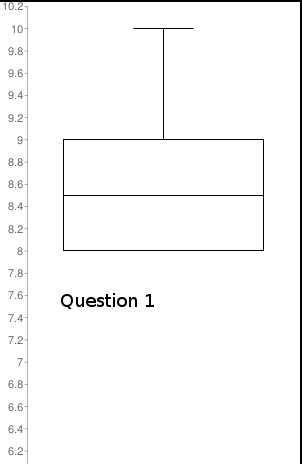
\includegraphics[scale=0.45]{images/q1}
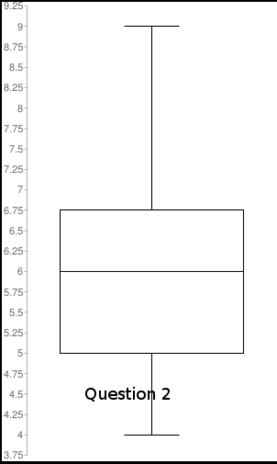
\includegraphics[scale=0.45]{images/q2}
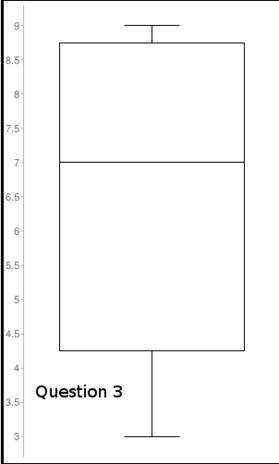
\includegraphics[scale=0.45]{images/q3}
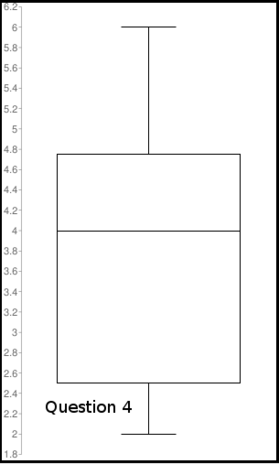
\includegraphics[scale=0.45]{images/q4}
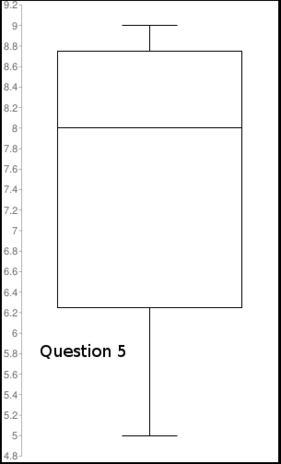
\includegraphics[scale=0.45]{images/q5}
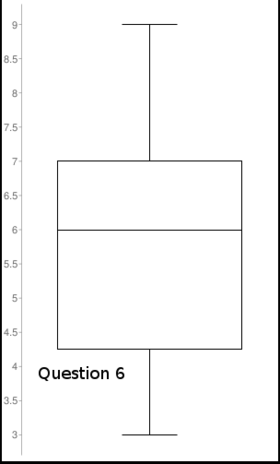
\includegraphics[scale=0.45]{images/q6}
\caption{Box plots which give a visual representation of answers}
\end{figure}
\end{center}
From this data it is clear that different people have varying opinions on the performance of the hybrid app which was developed. The answers to the questions as a whole generally give a positive response. It is apparent from the questions that users of the app do feel that the camera functionality is slower than a native app.

 \section{Resource Usage}
 When considering the hybrid mobile application it is also important to consider how much of the device's resources the app is using. For comparison the resource usage of Facebook has also been listed (this is because Facebook is a native app.)

 One of the resources which was compared was the amount of CPU, as shown in Figure X when Facebook was looking for events it used 6\% where as when the hybrid app which was developed was also 6\%. It does need to be considered that Facebook is significantly larger than the hybrid app which was created consequently the hybrid app uses more CPU for less data than Facebook. Figure 4.3 illustrates this.

\begin{figure}[H]
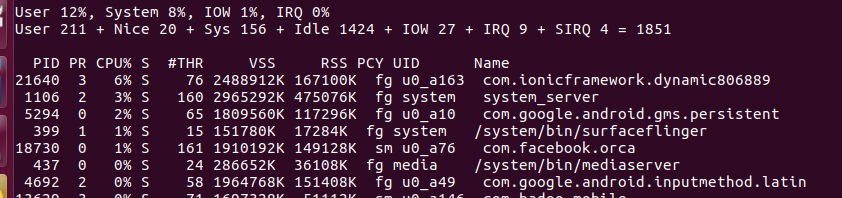
\includegraphics[scale=0.45]{images/ram2}
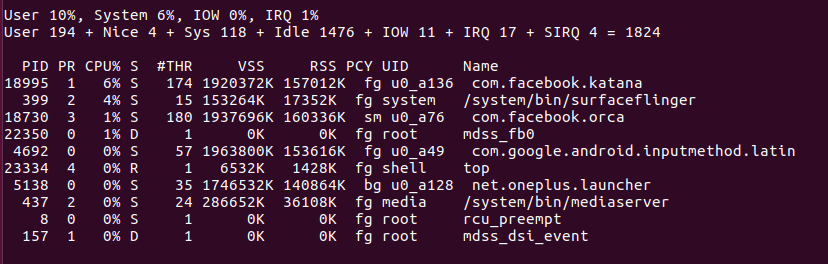
\includegraphics[scale=0.45]{images/ram3}
\caption{Images showing Facebook and Dynamic CPU.}
\end{figure}

The actual amount of storage the app uses is rather high when considering the app stores very little local data, this is mainly due to how ionic does caching. The app after being installed and a user going through different elements of the app uses 13.73MB of a device's storage which is rather large considering most things are stored on the back end rather than on the phone itself. 

\begin{center}
\begin{figure}[H]
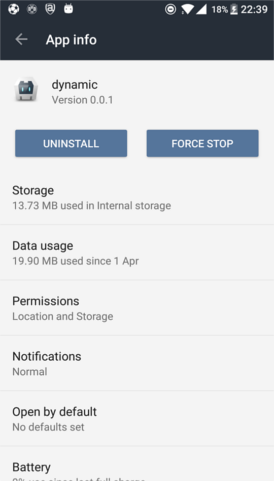
\includegraphics[scale=0.5]{images/usage}
\caption{Resource Usage}
\end{figure}
\end{center}

The amount of storage the app is using is a clear disadvantage to developing apps in a hybrid manner as developing apps in a native manner would give the developer more control over the amount of resources being used.

\section{Conclusion of testing}
The software development side to the project was a success as both the user acceptance testing and the unit tests passed. The user testing for actually determining whether hybrid apps are feasible alternatives to native apps was positive. From the multiple answers to the various questions asked it seems clear that users of the app are satisfied with it. Therefore, it would be reasonable to conclude that developing a mobile application in a hybrid manner is a feasible alternative to developing mobile applications in a native manner. When a comparison to Facebook has been made it does need to be considered that Facebook is a substantially larger system and has a lot more data. 


\chapter{Evaluation}

\section{Are hybrid apps feasible}
In determining whether hybrid apps are feasible alternatives to native apps it was important to consider both the advantages and disadvantages, not just of the actual hybrid app technologies but also of the actual development.

\subsection{Advantages}
\begin{itemize}
	\item Plugins allow for simple access to platform native APIs.
	\item Porting to multiple platforms is relatively simple.
	\item More developers are familiar with web technologies and languages as opposed to platform specific languages.
	\item As with native apps, they can be avaliable on platform stores such as Google Play Store and App Store.
	\item Developer only needs one language for multiple platforms.
	\item Useful debugging features such as Google Chrome's developer tools.
\end{itemize}
\subsection{Disadvantages}
\begin{itemize}
    \item Plugins do not give full control, such as issues with orientation on the camera plugin.
    \item Developer does not have full control over app's resource usage such as memory.
    \item Caching issues caused by the browser (which is displaying the app) even when developer tells app to not cache.
    \item Apps do generally seem slower for navigating around different pages as opposed to native apps. 
    \item Styling can be challenging, where as styling a native iOS app using xCode's story board is rather straightforward.

\end{itemize}
\subsection{Users thoughts}
As shown in the testing section the general thoughts on the mobile app by general users were positive. The majority of users felt that the hybrid app which was created, was as fast as a native app. This is rather interesting as there is generally a stigma in the development community that hybrid apps are significantly slower than native apps \cite{hybridcrap} yet the user testing was positive and many features of the app ran at the same speed as native apps (according to people who answered the questions). 

\subsection{Feasibility}
As the testing stage showed, it would be fair to state that hybrid apps are feasible alternative apps for the majority of applications. This is because users did not seem to notice hybrid apps being significantly slower than native apps even when using a device's platform specific features such as a camera. There are times where hybrid apps would not be feasible, such as for games or graphic heavy applications. Even though hybrid apps are feasible, there are negatives in that native features do not always work properly such as the issue with the camera orientation on Samsung tablets.

\section{Limitations of the system and future work}
In considering the system as a whole there is one potential problem. There is no way for sharing venues across multiple venue owners. Realistically at a big venue, it could be serveral people's jobs to create and promote events, however the app was designed in such a way that an email address and password would need to be shared if multiple people are creating events at the same venue.

For the mobile app to be released commercially there is some more work which would have to be carried out. This work would include:
\begin{itemize}
\item Improving the server - If the app was released commercially then the server would have to be able to handle multiple requests at once and more data. This means stress testing would have to be performed.
\item Push Notifications - Would add push notifications to tell users when upcoming events are happening.
\item Promotion - Appropriate flyers, web blogs, publications etc. would be produced to promote the app.
\item Email System - An email system would be set up. This would mean that a user would have to verify an account after creating it to ensure the email they provided was genuine.
\item Password Reset System - A system which would allow for users to reset their password if they have forgotten them.
\end{itemize} 
Another key thing which would have to be considered if the app was released in a commercial sense would be ethics. It would be important to have a terms and conditions which explains to the user exactly how their data would be used and that it would not be sold on. It would also be worth considering adding a minimum age to the app so that only users above a certain age can use the app. As the app does not have a profanity filter it would be important to ensure that young children aren't exposed to content which could be deemed offensive. Finally in relation to ethics it would possibly also be worth looking more into cyber bullying and how the app could aim to prevent cyber bullying.

\section{Evaluation of app development itself}
For the most part using the Scrum methodology worked well as it allowed for each different function of the app to be broken down into a story. At first it was rather difficult to estimate how long each story would take but after implementing a few stories, estimation became much easier.

Using a plan driven methodology could have also worked well for developing the app and if a plan driven methodology had been used, then a PHP framework would have probably been used rather than having lots of different PHP files. 

The app development itself went rather smoothly once the basics of AngularJS had been learned. There were some problems which were encountered such as issues with caching and issues with converting postcodes to latitude, longitude locations. These technical challenges were resolved mainly through research and looking at various sources online.      
\section{Requirements correctly identified}
As this project was an investigation as well as the development of the app, it was important that the development was carried out to aid the investigation. In this case it certainly appears that the requirements were indeed correctly identified as the development of the app enabled a judgement about whether hybrid apps are feasible alternatives to native apps to be made.

There were more requirements which could have been added which would have allowed for a more solid judgement to be made. These requirements would have involved using more platform native APIs so features such as push notifications along with access to a device's email could have been added to aid the judgement.
\section{Design decisions}
There were some good decisions made in relation to the design of the app. Using ionic was certainly a good idea as it encourages the MVC framework and therefore means that the code created was easy to read and easy to understand. The decision to create all of the PHP API files manually was a poor decision  as it led to lots of time being spent on the actual development of the PHP files and this time could have been better utilised elsewhere.
\section{Project aims achieved}
The projects aims were achieved as I established that hybrid applications are feasible alternatives to native applications for the majority of purposes. The aims were achieved by correctly identifying requirements which enabled a sound judgement to be made.
\subsection{What would be done differently}
When considering the project with hindsight, a few things would be done differently to make the project more effective. First of all the back end would be created using a framework as this would allow for fewer PHP files and less code repetition. Also SASS would be used as opposed to CSS as SASS would give the developer more flexibility in styling the app.

\subsection{Conclusion}
The project was most certainly a success in that it proved that hybrid apps are feasible alternatives to native apps. As well as this, through the actual development of a hybrid app, the advantages and disadvantages of hybrid apps were made clear.

Whilst hybrid apps are feasible alternatives they do have some way to go especially in terms of giving the developer full control over a device's native features such as a camera. For such things to happen then hybrid apps probably need to become more common. In terms of making hybrid apps more common, developers need to be made aware of exactly what hybrid apps are and when it can be useful to use them. 

% add any additional chapters here

\setemptyheader
\addcontentsline{toc}{chapter}{Appendices}
\chapter*{Appendices}
\pagebreak

% start the appendix - sets up different numbering
\fancypagestyle{plain}{%
%\fancyhf{} % clear all header and footer fields
\fancyhead[L]{\textsl{Appendix\ \thechapter}}
\fancyhead[R]{\textsl{\leftmark}}}

\appendix
\fancyhead[L]{\textsl{Appendix\ \thechapter}}
\fancyhead[R]{\textsl{\leftmark}}
\fancyhead[C]{}
\fancyfoot[C]{\thepage}
\renewcommand{\headrulewidth}{0.4pt}
\renewcommand{\chaptermark}[1]{\markboth{#1}{}}

\fancyhead[L]{\textsl{Appendix\ \thechapter}}
\fancyhead[R]{\textsl{\leftmark}}
\fancyfoot[C]{{\thepage} of \pageref{LastPage}}

% include any appendices here
\chapter{Third-Party Code and Libraries}

If you have made use of any third party code or software libraries, i.e. any code that you have not designed and written yourself, then you must include this appendix. 

As has been said in lectures, it is acceptable and likely that you will make use of third-party code and software libraries. The key requirement is that we understand what is your original work and what work is based on that of other people. 

Therefore, you need to clearly state what you have used and where the original material can be found. Also, if you have made any changes to the original versions, you must explain what you have changed. 

As an example, you might include a definition such as: 

Apache POI library � The project has been used to read and write Microsoft Excel files (XLS) as part of the interaction with the client�s existing system for processing data. Version 3.10-FINAL was used. The library is open source and it is available from the Apache Software Foundation 
\cite{apache_poi}. The library is released using the Apache License 
\cite{apache_license}. This library was used without modification. 

\chapter{Ethics Submission Assessment}
\section{Ethics Submission Assessment reference number: 6663}
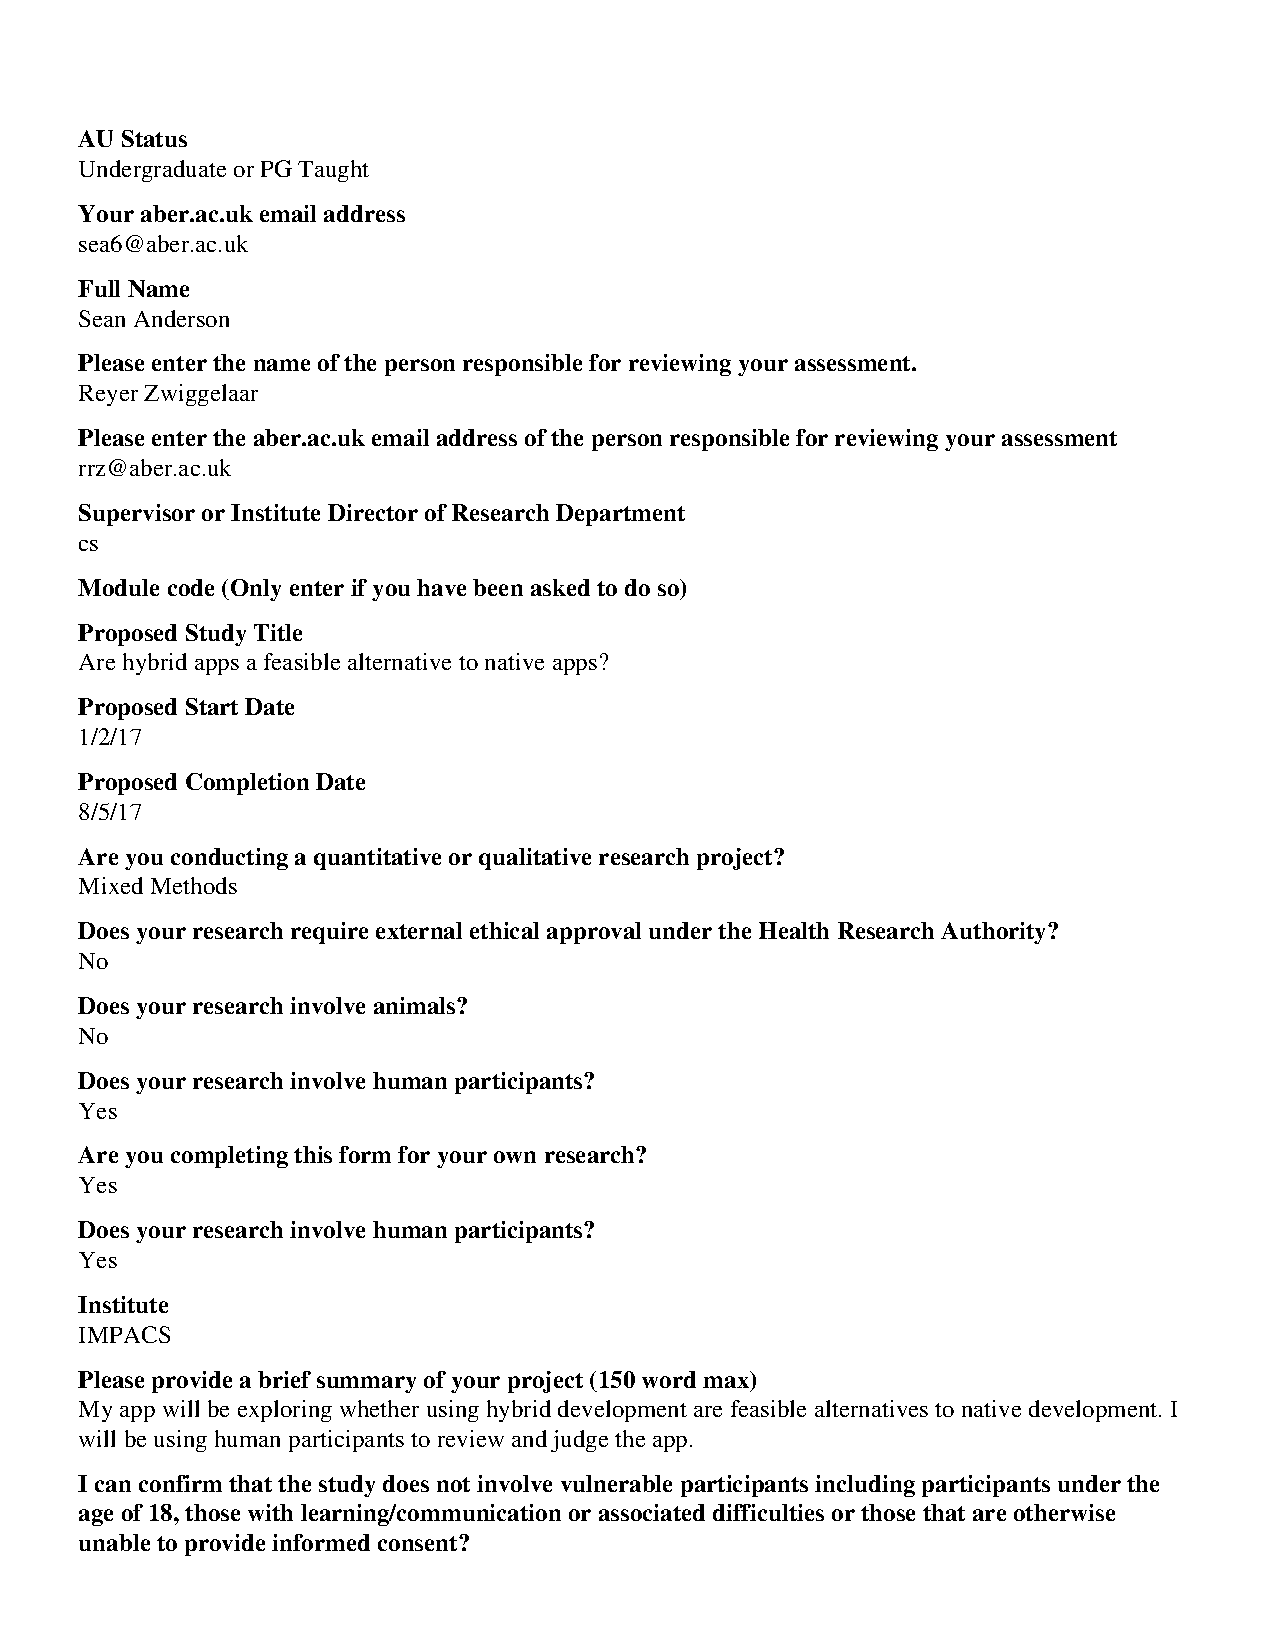
\includegraphics[scale=0.6]{6663.pdf}
\chapter{Questionaire }
\section{Registration AngularJS Controller (register.js)}
\begin{verbatim}
angular.module('register.controllers', [])
.controller('RegisterCtrl', function($scope, $ionicModal, 
$http, $state, $ionicPopup) {
  var apiReturns;
  var api = "http://seananderson.co.uk/api/listgenre.php";
  $http.get(api).then(function(res) {
    var length = (res['data']).length;
    var select = angular.element(document.querySelector('#genre'));
    for (i=0;i<length;i++) {
      select.append('<option>' + res['data'][i] + '</option>');
    }
  })

   // Form data for the login modal
  $scope.register = {};

  //Generic popup as there may need to be 
  //multiple popups for this page. Code is based of 
  //ionic documentation for popup.
  popUp = function(title, message) {
    var alertPopup = $ionicPopup.alert({
      title: title,
      template: message
    });
    alertPopup.then(function(res) {
    });
  }

  //Return to login page i.e user has decided they dont need to register.
  $scope.returnToLogin = function() {
    $state.go('login');
  }

  //Function which checks to make sure all fields 
  //on the form have been filled in.
  $scope.checkFields = function() {
    if ($scope.register.fName==undefined){
      popUp("Field Missing", "First Name Field Was Not Entered");
      return false;
    }

    if ($scope.register.lName==undefined) {
      popUp("Field Missing", "Last Name Field Was Not Entered.");
      return false;
    }

    if ($scope.register.email==undefined) {
      popUp("Field Missing", "Email address was not entered.");
      return false;
    }

    if ($scope.register.password==undefined) {
      popUp("Field Missing", "Password was not entered");
      return false
    }

    if ($scope.register.cPassword==undefined) {
      popUp("Field Missing", "Confirmation password was not entered");
      return false;
    }

    if ($scope.register.pCode==undefined) {
      popUp("Field Missing", "Postcode was not entered");
      return false;
    }

    if ($scope.register.dName==undefined) {
      popUp("Field Missing", "Display Name was not entered");
      return false;
    }

    if ($scope.register.userType==undefined) {
      popUp("Field Missing", "User Type was not selected.");
      return false;
    }

    if ($scope.register.genre===undefined) {
      popUp("Field Missing", "You haven't selected your 
      favoruite genre of music.");
      return false;
    }
    else {
      return true;
    }
  }

  //Function for regsitering genre of music which user likes.
  $scope.registerGenre = function() {
    var api = "http://seananderson.co.uk/api/registergenre.php";
    $scope.register.genre.forEach(function(genre) {
    var data = {
      email: $scope.register.email,
      genre: genre
      }
      $http.post(api, data).then(function(res) {
        console.log(res);
      })
    })
  }

  //Function which valides that the users postcode they have entered is correct.
  $scope.checkPostcode = function() {
    var postcode = $scope.register.pCode;
    $scope.register.pCode = postcode.replace(/[\s]/g, '');
    if ($scope.register.pCode.length!=6) {
      if ($scope.register.pCode.length!=7) {
        if ($scope.register.pCode.length!=8) {
          popUp("Postcode is incorrect length must be 6,7 or 8 characters.")
          return false;
        }
      }
    }
    return true;
  }

  $scope.checkPassword = function() {
    if ($scope.register.password.length<6) {
      popUp("Password Invalid", "Password length must be 6 or greater.");
      return false;
    }
    return true;
  }


  //Function for when the user clicks the validation button.
  $scope.doRegistration = function() {
    //Checks all necessary fields have values.
    if ($scope.checkFields()==false){
      return;
    }
    if($scope.checkPostcode()==false) {
      return;
    }

    if ($scope.checkPassword()==false) {
      return;
    }

    //Validates email address is a new email.
    var api= "http://seananderson.co.uk/api/checkemail.php";
    var data = {
      email: $scope.register.email
    }
    $http.post(api,data).then(function(res) {
      var apiResponse = JSON.stringify(res);
      var correct = "This email is fine"
      if (apiResponse.includes(correct)) {
        if ($scope.register.password==$scope.register.cPassword) {
          if($scope.register.userType=="Music Lover") {
            var type = 1;
          }
          else if ($scope.register.userType=="Artist") {
            var type = 2;
          }
          else if ($scope.register.userType=="Venue Owner") {
            var type = 3;
          }
          else {
            popUp('No User Type', 'No user type has been selected.' );
          }
          var api = "http://seananderson.co.uk/api/displayname.php";
          var data = {
            dName: $scope.register.dName
          }

          //Checks Display Name isn't already being used.
          $http.post(api, data).then(function(res) {
            apiReturns = JSON.stringify(res);
            var incorrect = "This user name has already been used";
            if (apiReturns.includes(incorrect)) {
              popUp('This display name has already been 
              used please choose another 
              display name.');
            }
            else {
              var api = "http://seananderson.co.uk/api/register.php";
              var data = {
                firstName: $scope.register.fName,
                lastName: $scope.register.lName,
                email: $scope.register.email,
                type: type,
                password: $scope.register.password,
                postcode: $scope.register.pCode,
                dName: $scope.register.dName
              }
              $http.post(api, data).then(function(res){
                apiReturns = JSON.stringify(res);
                if (apiReturns.includes('New user added succesfully')>=0) {
                  localStorage.setItem('email', $scope.register.email);
                  localStorage.setItem('dName', $scope.register.dName);
                  if ($scope.registerGenre!=undefined) {
                    $scope.registerGenre();
                  }
                  $state.go('app.profile');
                  popUp('Welcome', 'Welcome to Dynamic please 
                  fill in your profile page and then 
                  follow some users');
                }
              })
            }
          })
        }
        else {
          popUp('Passwords do not match', 'The confirmation 
          password is not the same as the initial 
          password you entered');
        }
      }
      else {
        popUp("Email is not valid", "Please use a valid 
        email address which hasn't 
        already been used");
      }
    })
  }
})
\end{verbatim}

\section{Registration API (register.php)}
\begin{verbatim}
<?php
header('Access-Control-Allow-Origin: *');
header("Access-Control-Allow-Headers: Origin, 
X-Requested-With, Content-Type, Accept");
header('Access-Control-Allow-Methods: GET, POST, PUT');

include "config.php";
$connection = new mysqli($server, $dbuser, $dbpass, $dbname);

if ($connection->connect_error) {
    die ("Connection to the database failed." 
    . $connection->connect_error);
}

if ($_SERVER['REQUEST_METHOD'] == 'POST' && empty($_POST))
    $_POST = json_decode(file_get_contents('php://input'), true);

$firstName = mysqli_real_escape_string($connection, $_POST['firstName']);
$lastName = mysqli_real_escape_string($connection, $_POST['lastName']);
$email = mysqli_real_escape_String($connection, $_POST['email']);
$type = mysqli_real_escape_String($connection, $_POST['type']);
$dName = mysqli_real_escape_String($connection, $_POST['dName']);
$password = mysqli_real_escape_String($connection, $_POST['password']);
$password = password_hash($password, PASSWORD_DEFAULT);
$postcode = mysqli_real_escape_String($connection, $postcode);

if (filter_var($email, FILTER_VALIDATE_EMAIL)) {
    $sql = "INSERT into users (firstname, lastname, email, type, 
    displayname, password, postcode)
    VALUES ('$firstName', '$lastName', '$email', 
    $type, '$dName', '$password', '$postcode')";

    if ($connection->query($sql) === TRUE) {
        echo "New user added succesfully";
    } 
    else {
        echo "Error: " . $sql . "</br>" . $conn->error;
    }
}

else {
    echo "Email is not valid";
}

$connection->close();
?>
\end{verbatim}

\section{Unit Tests for Login and Register}
\begin{verbatim}
describe('LoginController', function() {

    var controller, 
        loginServiceMock,
        stateMock,
        ionicPopupMock;

    beforeEach(module('app'));  

    describe('#doLogin', function() {

        // TODO: Call doLogin on the Controller

        it('should call login on dinnerService', function() {
            expect(loginServiceMock.login).toHaveBeenCalledWith('sea6@aber.ac.uk', 'b261la'); 
        });

        describe('when the login action is performed,', function() {
            it('if successful, should change state to home', function() {

                // TODO: Mock the login response from DinnerService

                expect(stateMock.go).toHaveBeenCalledWith('app.home');
            });

            it('if unsuccessful, should show a popup', function() {

                // TODO: Mock the login response from DinnerService

                expect(ionicPopupMock.alert).toHaveBeenCalled();
            });
        });
    })
});
\end{verbatim}

\section{Login Unit Test (logintest.js)}
\begin{verbatim}
describe('LoginCtrl', function() {

    var controller, 
        loginMock,
        stateMock,
        ionicPopupMock;
    
    beforeEach(module('app'));

    beforeEach(module('#'));  

    describe('#doLogin', function() {


        it('Should Login using correct details', function() {
            expect(loginMock.doLogin).toHaveBeenCalledWith('sea6@aber.ac.uk', 'b261la'); 
        });

        describe('when the login action is performed,', function() {
            it('if successful, should change state to home', function() {
                expect(stateMock.go).toHaveBeenCalledWith('app.home');
            });

            it('if unsuccessful, should show a popup', function() {

                expect(ionicPopupMock.alert).toHaveBeenCalled();
            });
        });
    })

    describe('#register', function(){

        it('Should go to register screen', function(){
             expect(stateMock.go).toHaveBeenCalledWith('register');
        })
    })


});
\end{verbatim}



\fancypagestyle{plain}{%
   \fancyhead{} %[C]{Annotated Bibliography}
   \fancyfoot[C]{{\thepage} of \pageref{LastPage}} % except the center
   \renewcommand{\headrulewidth}{0pt}
   \renewcommand{\footrulewidth}{0pt}
}

\setemptyheader

\nocite{*} % include everything from the bibliography, irrespective of whether it has been referenced.

% the following line is included so that the bibliography is also shown in the table of contents. There is the possibility that this is added to the previous page for the bibliography. To address this, a newline is added so that it appears on the first page for the bibliography. 
\addcontentsline{toc}{chapter}{Annotated Bibliography} % Adds References to contents page

%
% example of including an annotated bibliography. The current style is an author date one. If you want to change, comment out the line and uncomment the subsequent line. You should also modify the packages included at the top (see the notes earlier in the file) and then trash your aux files and re-run. 
%\bibliographystyle{authordate2annot}
\bibliographystyle{IEEEannot}
\renewcommand{\bibname}{Annotated Bibliography} 
\bibliography{References/references} % References file


\end{document}
